\section{Additional Results}
\label{app:additional-results}

In this section, we present additional results and ablations from our experimental evaluation.

\subsection{Ablating the Maximum Sample Length}
\label{app:additional-results:max-sample-length-ablation}

\begin{figure}
    \begin{subfigure}[t]{\textwidth}
        \begin{center}
            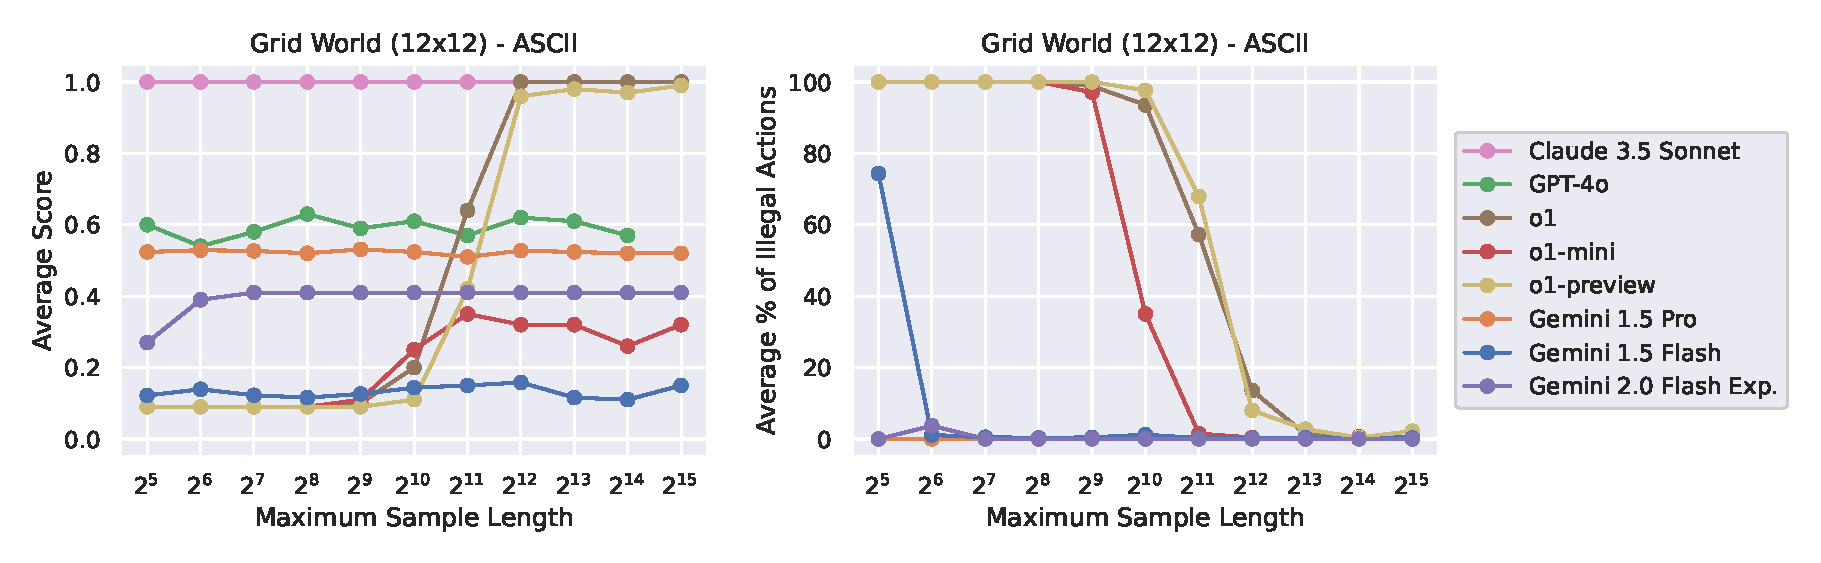
\includegraphics[width=\textwidth]{figures/grid_world_12x12_txt_max_sample_length.eps}
        \end{center}
        \caption{ASCII observations}
    \end{subfigure}
    \par\bigskip
    \begin{subfigure}[t]{\textwidth}
        \begin{center}
            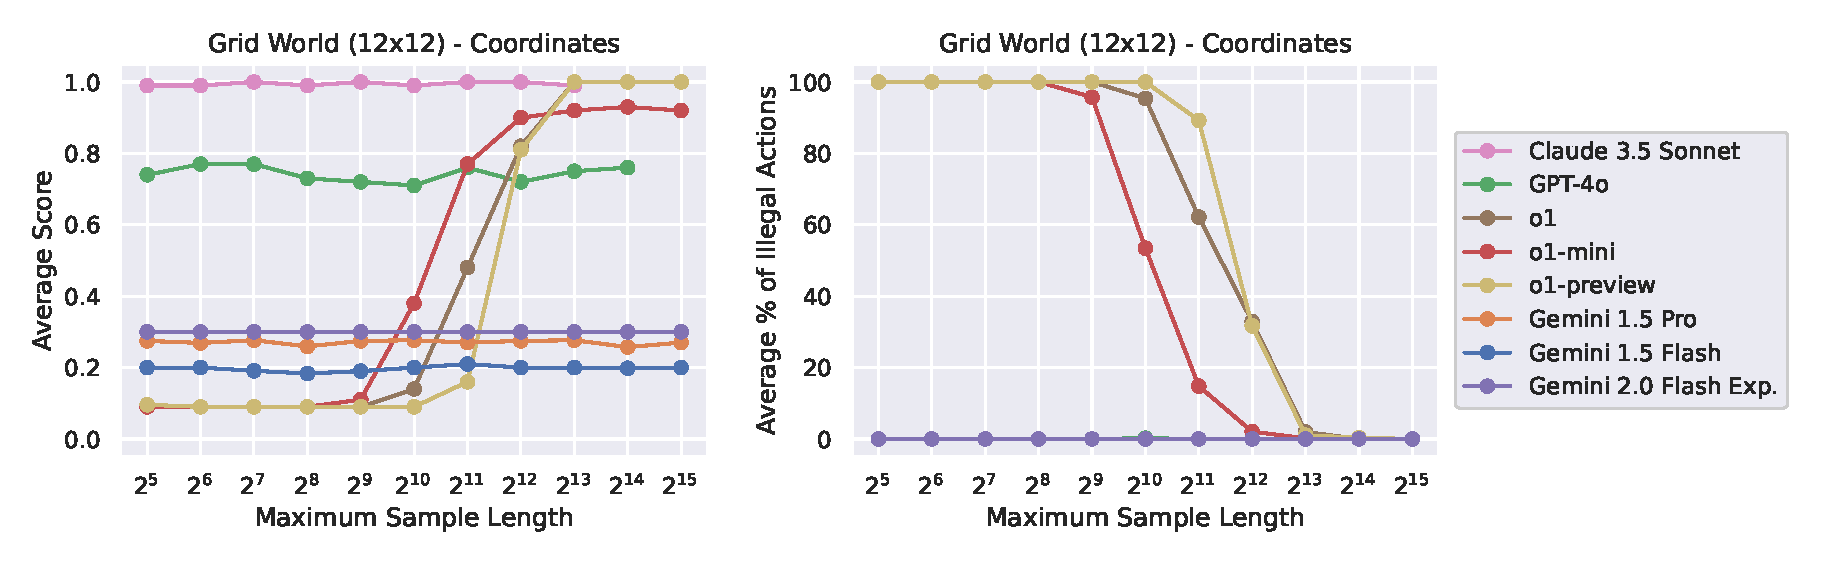
\includegraphics[width=\textwidth]{figures/grid_world_12x12_coords_max_sample_length.eps}
        \end{center}
        \caption{Coordinate observations}
    \end{subfigure}
    \par\bigskip
    \begin{subfigure}[t]{\textwidth}
        \begin{center}
            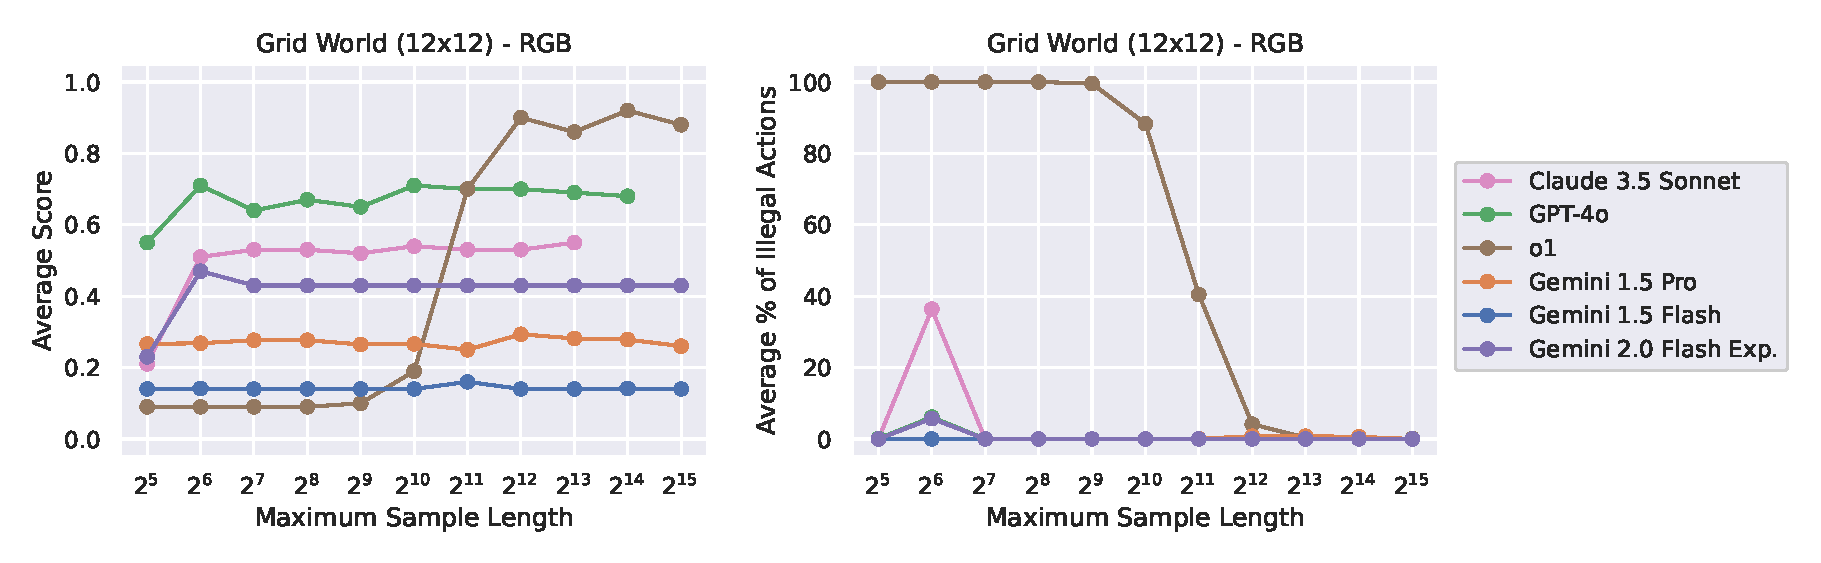
\includegraphics[width=\textwidth]{figures/grid_world_12x12_rgb_max_sample_length.eps}
        \end{center}
        \caption{RGB observations}
    \end{subfigure}
    \caption{
        Ablating the maximum sample length for all three observation types (ASCII, coordinates, and RGB images) of the grid world navigation task with $1$ demonstration episode (the left panels show the average score, the right panels show the percentage of illegal actions).
        As expected, $32$ output tokens are sufficient for \claude{}, \gpt{}, \flash{}, and \pro{} to achieve their best performance on the task.
        In contrast, \mini{} and \preview{} require between $4096$ and $8192$ output tokens to achieve their best performance.
        With less than $8192$ output tokens, the o1 models do not have enough internal ``reasoning tokens'' at their disposal to produce an output, which can be seen by the sharp increase in the percentage of illegal actions in the right panels.
        Note that \mini{} and \preview{} are text-only models and therefore cannot process RGB image observations.
    }
    \label{fig:sample-length-ablation}
\end{figure}

The o1 family of models tends to generate (long) internal ``reasoning traces'' before returning an output.
Thus, if the maximum sample length is not large enough, these models may not have enough ``reasoning tokens'' and therefore do not produce an output (in which case the API returns an empty sample).
Since we want to report each model's best performance on our benchmark, we therefore ablate the maximum number of sample tokens and choose the configuration that trades off good performance and low cost (since, after a certain point, more tokens generally do not improve performance but only increase the cost).
The maximum sample length also has an impact on the other models, particularly when using chain-of-thought reasoning, but a relatively low sample length typically suffices for our tasks (unlike the o1 models which require large maximal sample length).

To that end, \cref{fig:sample-length-ablation} shows our ablation of the maximum sample length for \claude{}, \gpt{}, \mini{}, \preview{}, \flash{}, and \pro{} on all three observation types (ASCII, coordinates and RGB) for the grid world navigation task with $1$ demonstration episode.
\cref{fig:sample-length-ablation} shows the average score over $100$ evaluation episodes for maximum sample lengths from $32$ to $32768$ tokens (\claude{} only supports $8192$ output tokens and \gpt{} only supports $16384$ output tokens).
Unsurprisingly, the performance of \claude{}, \gpt{}, \flash{}, and \pro{} is largely unaffected by the number of sample tokens, \ie even $32$ tokens are sufficient to achieve their best performance (with the exception of \claude{} and \gpt{} on RGB observations, where they benefit from having $64$ tokens).
This is in stark contrast with \mini{} and \preview{}, which require between $4096$ and $8192$ output tokens to achieve their optimal performance (with a very steep degradation below $4096$).
To verify whether this sharp rise in performance is actually due to the model not generating a valid action, \cref{fig:sample-length-ablation} also visualizes the average percentage of illegal actions per episode over the maximum sample length, which (inversely) correlates very strongly with performance for the o1 models.
We therefore set the maximum sample length to $8192$ for the o1 models as a tradeoff between cost and performance (the maximum for \preview{} is $32768$, the maximum for \mini{} is $65536$~\citep{openai2024reasoning}).
This should enable the o1 models to achieve their best performance on our benchmark --- even though they do so at a much higher (computational) cost than the other models.


\subsection{Replaying a Demonstration Episode}
\label{app:additional-results:replay}

In-context imitation learning requires several different skills, one of which is being able to locate and retrieve the relevant demonstration(s) from the context.
We therefore conduct a ``sanity check'' experiment where we provide a single demonstration episode and ``replay'' the exact same episode for evaluation (akin to a multimodal sequence copying task).
Thus, for every step, the model only has to find the correct location in the demonstration episode in its context and reproduce its corresponding action.
Accordingly, we slightly change the evaluation setup since the next observation (both action and next state) in the evaluation trajectory is always determined by the demonstration episode and not by the action generated by the model (\ie we perform teacher forcing rather than a dynamic evaluation).
As a result, we are not interested in a model's return but in how often it manages to match the action from the demonstration episode.
Like in our other experiments, we evaluate $100$ different episodes.
For the sake of simplicity, we do not use chain-of-thought prompting, do not show the legal actions in the prompt, and only consider a single demonstration episode.
Other than that, we leave the prompt the same as in our default experimental setup (\ie including the same preamble and separator).

\cref{fig:replay-atari,fig:replay-chess,fig:replay-crossword,fig:replay-dm-control,fig:replay-grid-world,fig:replay-tic-tac-toe} show the average action replay accuracy per evaluation step for all frontier models on all six environments (for all state representation formats separately).
We observe that models are generally capable of replaying the demonstration episodes, with slightly lower performance deeper into the episode.
The significant exception is \mini{} which struggles with the replay task in most settings.
Similarly, \flash{} fails to replay the actions for tic-tac-toe with RGB observations.
Note that, in theory, the observation type is irrelevant for this task since the models could just count the number of observations in the evaluation trajectory and select the corresponding action in the demonstration trajectory.

\begin{figure}
    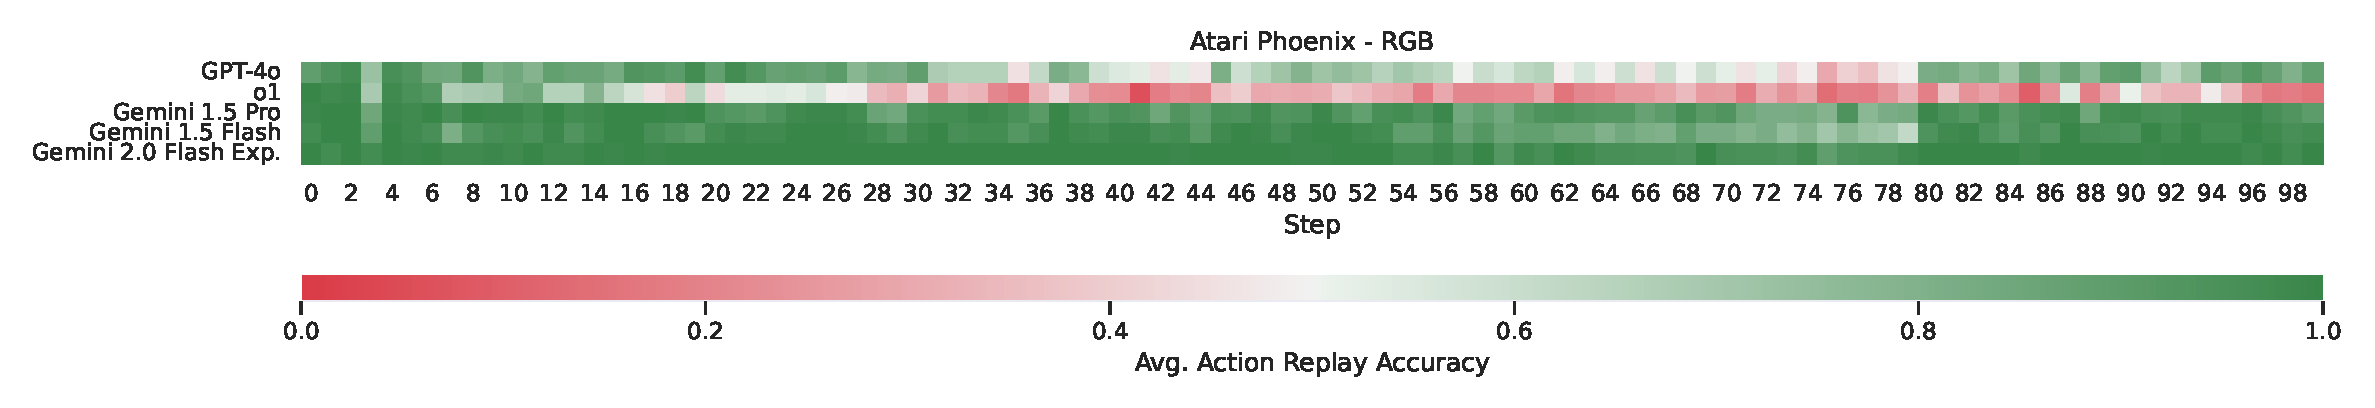
\includegraphics[width=\textwidth]{figures/atari_phoenix_rgb_replay}
    \caption{
        Replaying the demonstration episode for the Phoenix game (with RGB observations) from Atari $2600$.
        The color visualizes the models' average accuracy when attempting to replay the action for a given step.
        The Gemini 1.5 models generally perform well at replaying the demonstrations, regardless of the step, though they show a slight degradation in performance towards the $80$-step mark, from which they immediately recover again.
        The performance of \gpt{} shows a slightly higher degradation towards step $80$, but also immediately recovers thereafter.
        Note that \claude{} cannot process more than $100$ images at a time, so we cannot evaluate it on this task.
        Similarly, \mini{} and \preview{} are text-only and, therefore, cannot process RGB observations.
    }
    \label{fig:replay-atari}
\end{figure}

\begin{figure}
    \begin{subfigure}[t]{\textwidth}
        \begin{center}
            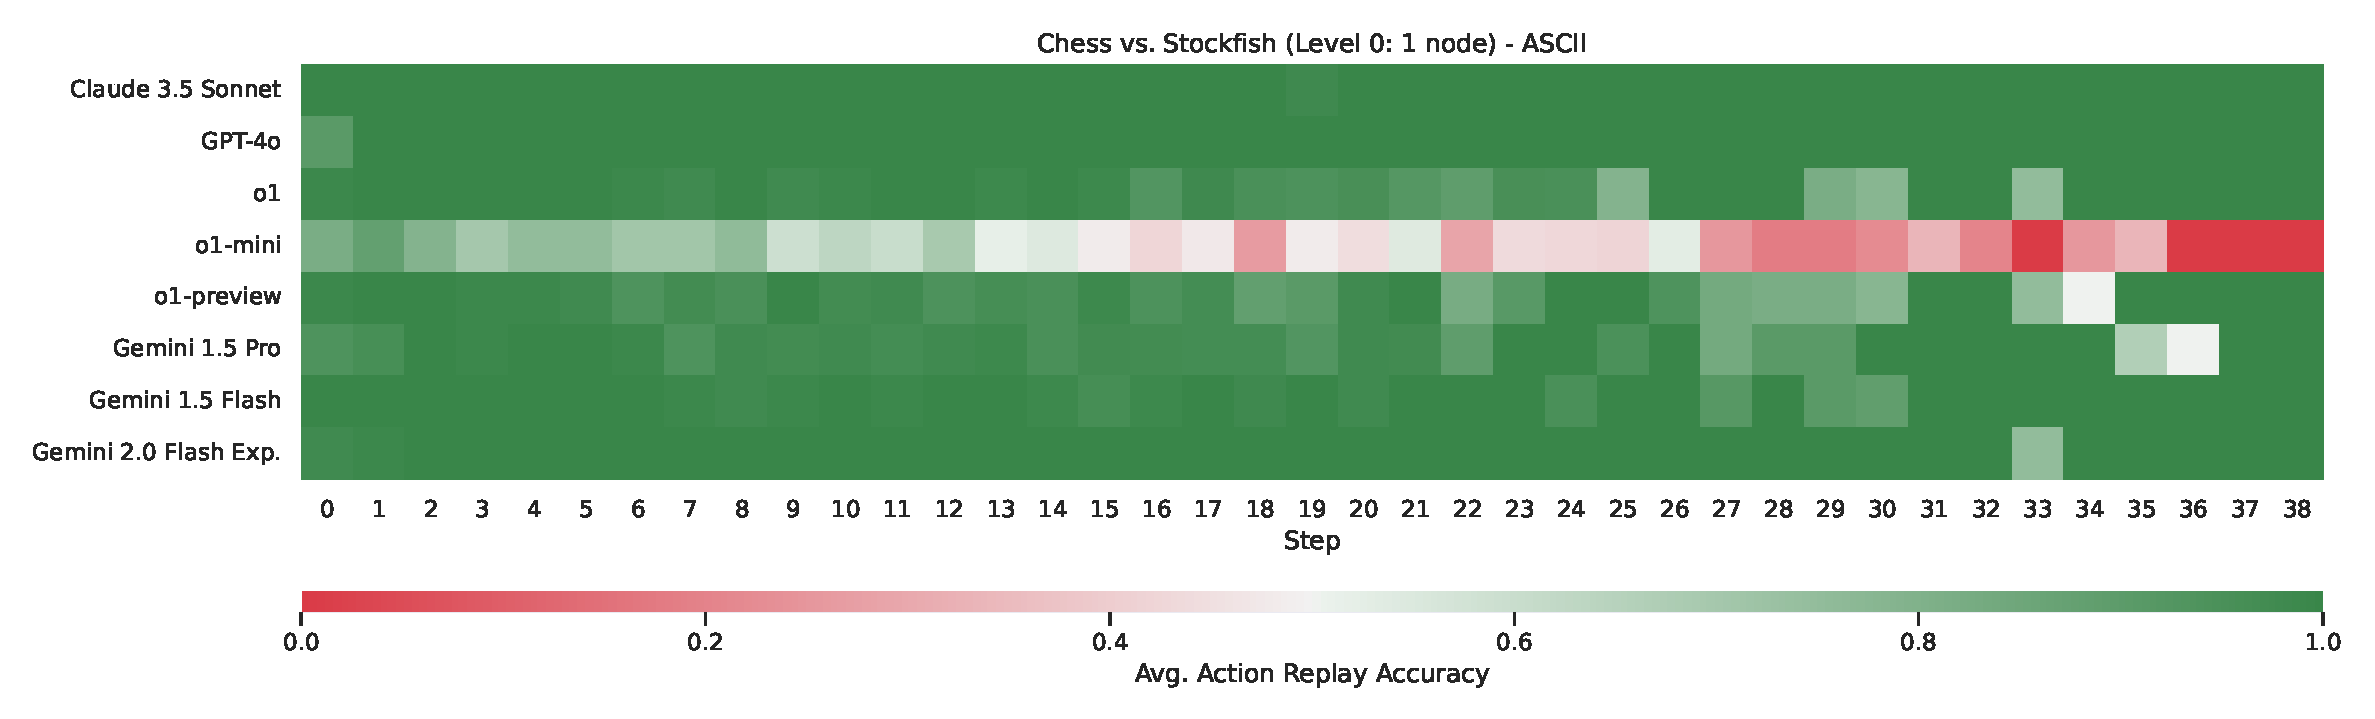
\includegraphics[width=0.9\textwidth]{figures/chess_txt_replay.eps}
        \end{center}
        \vspace{-8pt}
        \caption{ASCII observations}
    \end{subfigure}
    \par\bigskip
    \begin{subfigure}[t]{\textwidth}
        \begin{center}
            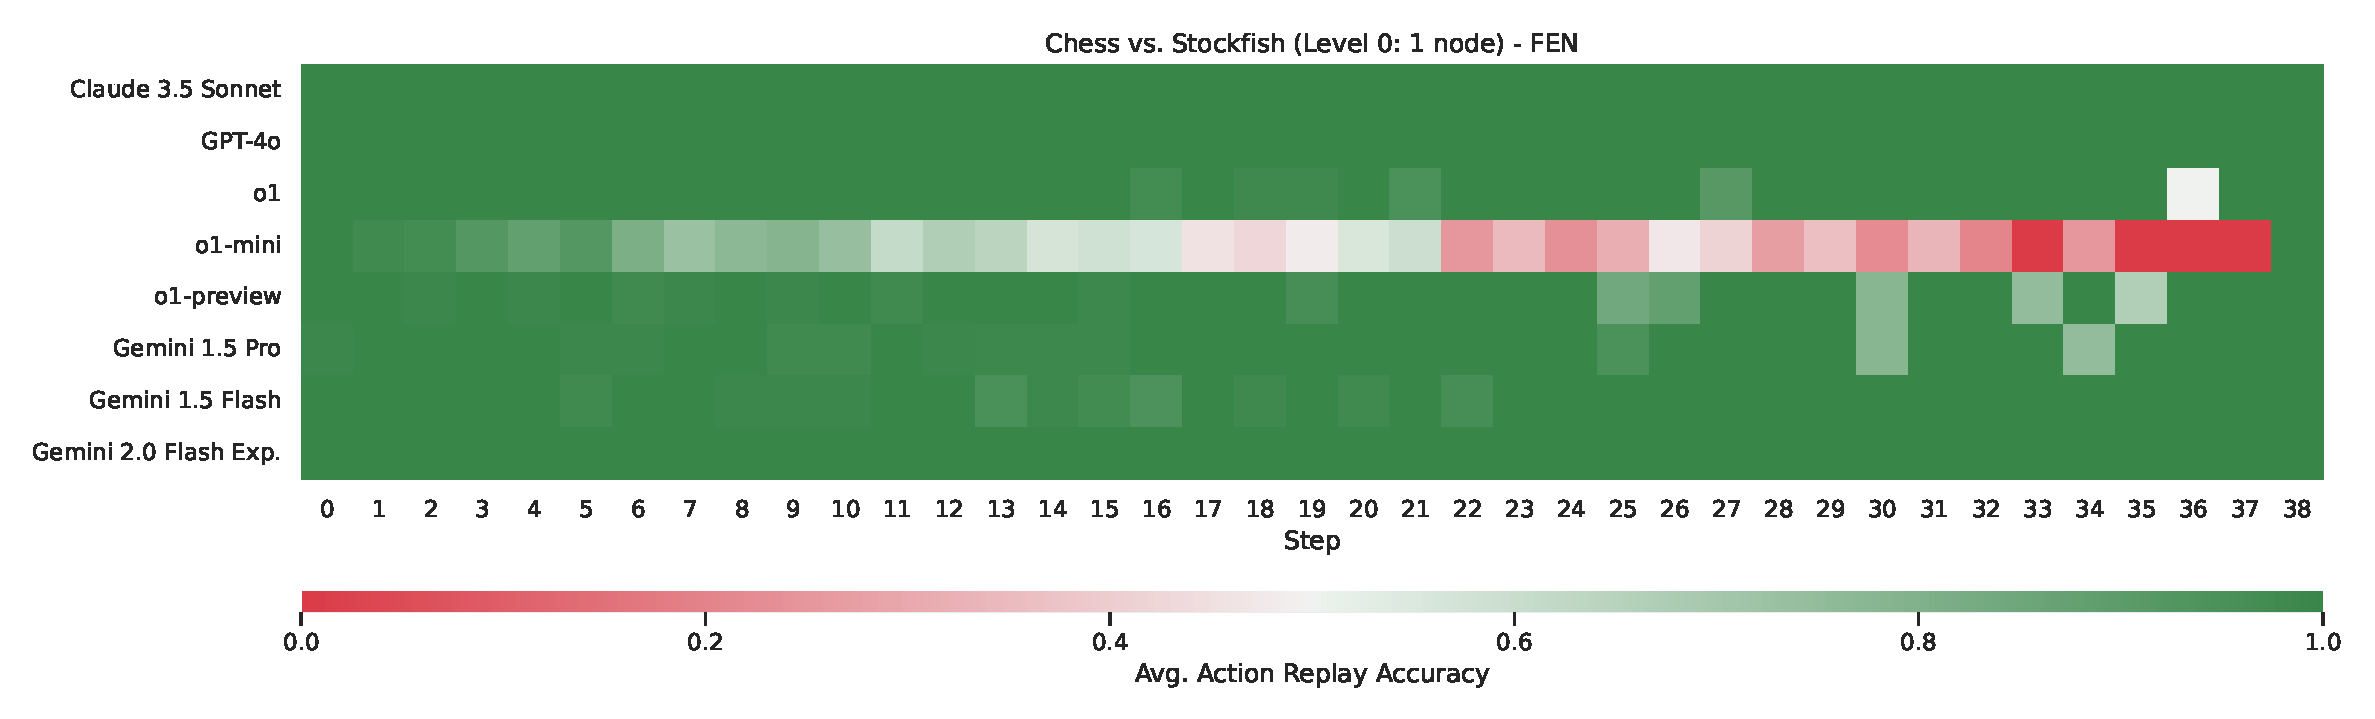
\includegraphics[width=0.9\textwidth]{figures/chess_fen_replay.eps}
        \end{center}
        \vspace{-8pt}
        \caption{FEN observations}
    \end{subfigure}
    \par\bigskip
    \begin{subfigure}[t]{\textwidth}
        \begin{center}
            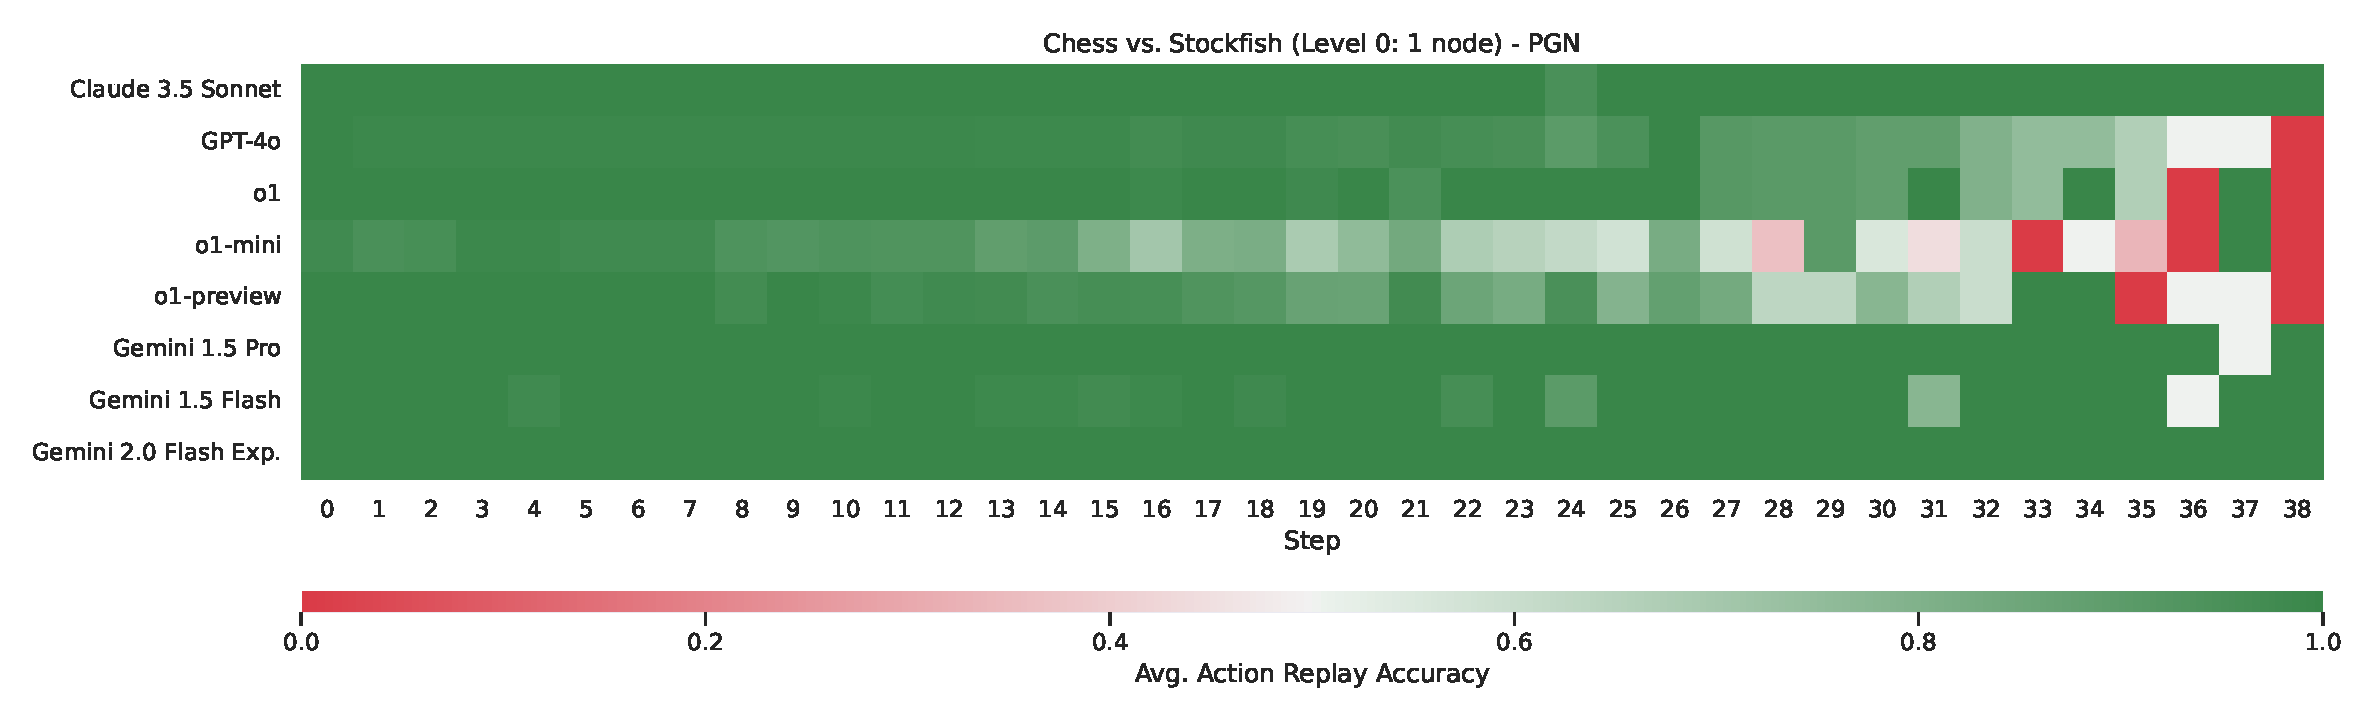
\includegraphics[width=0.9\textwidth]{figures/chess_pgn_replay.eps}
        \end{center}
        \vspace{-8pt}
        \caption{PGN observations}
    \end{subfigure}
    \par\bigskip
    \begin{subfigure}[t]{\textwidth}
        \begin{center}
            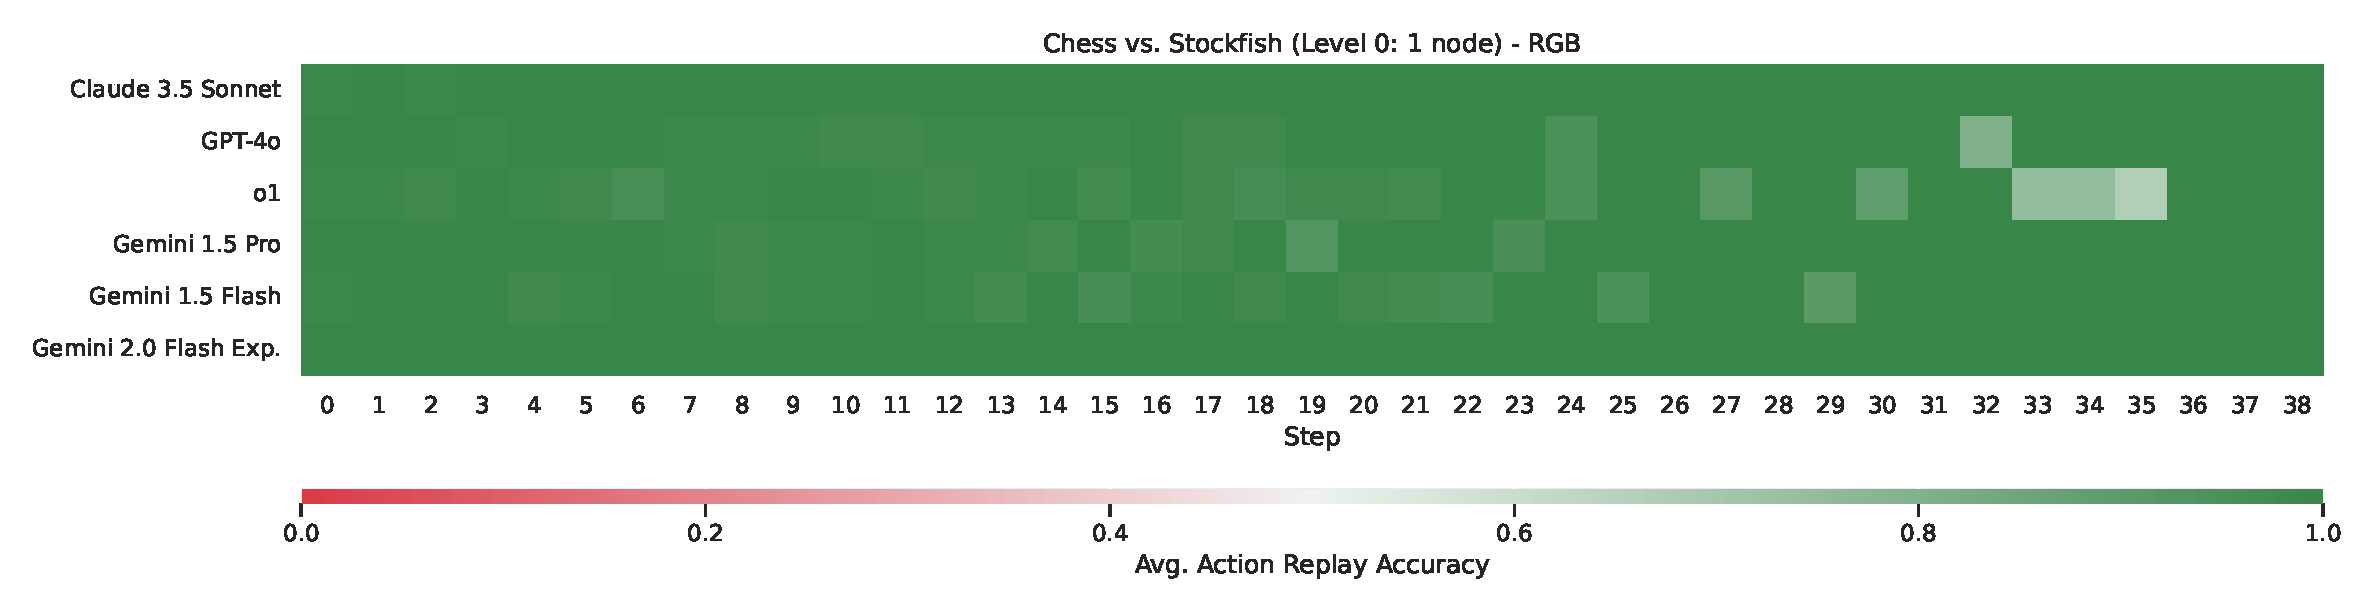
\includegraphics[width=0.9\textwidth]{figures/chess_png_replay.eps}
        \end{center}
        \vspace{-8pt}
        \caption{RGB observations}
    \end{subfigure}
    \caption{
        Replaying the demonstration episode for the different observation types from our chess environments.
        The color visualizes the models' average accuracy when attempting to replay the action for a given step.
        All models generally perform well across all observation types, except for \mini{}, which shows a strong performance degradation towards the end of the episode across all three observation text observation types (recall that \mini{} and \preview{} are text-only models, and, therefore, cannot process RGB images).
        With the exception of \claude{}, all models struggle (to varying degrees) to replay the last few actions with PGN observations.
    }
    \label{fig:replay-chess}
\end{figure}

\begin{figure}
    \begin{center}
        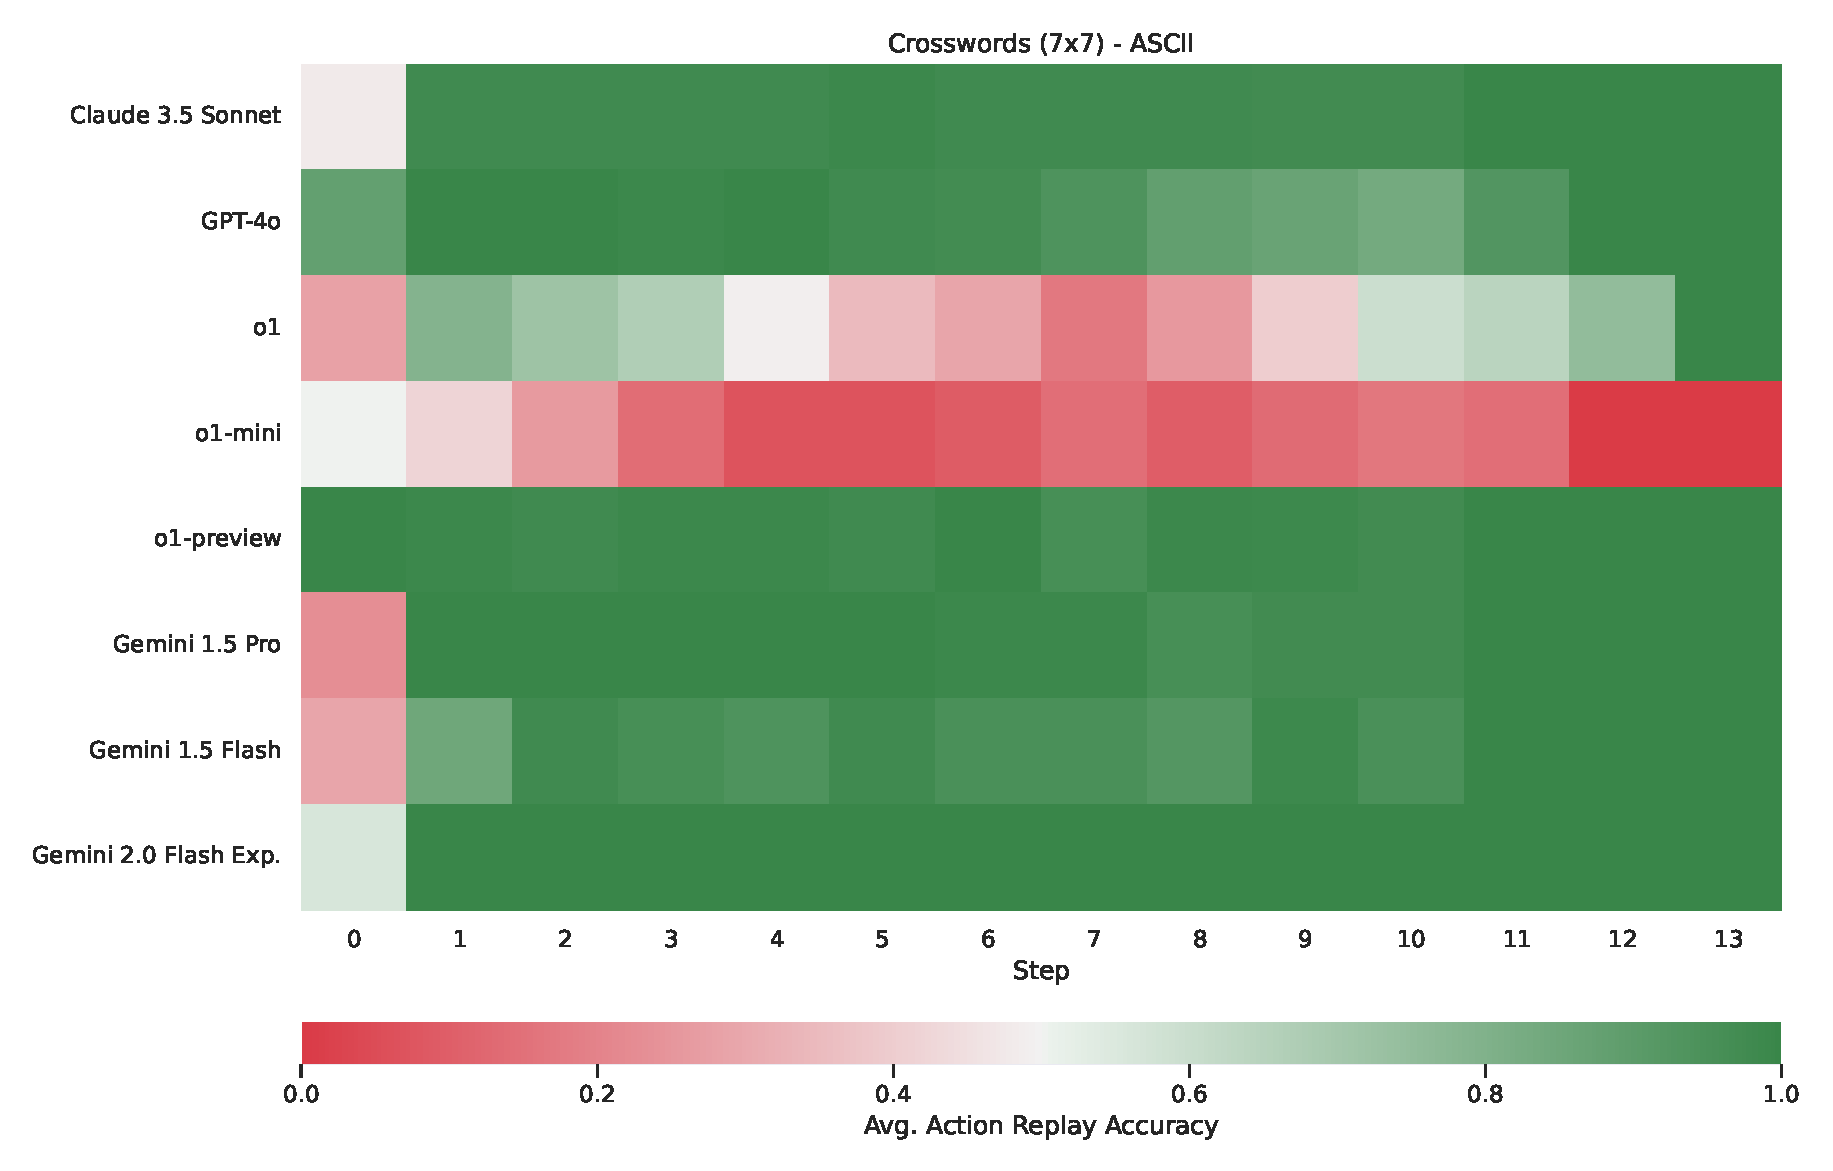
\includegraphics[width=0.6\textwidth]{figures/crossword_txt_replay.eps}
    \end{center}
    \caption{
        Replaying the demonstration episode for our crossword environment with ASCII observations.
        The color visualizes the models' average accuracy when attempting to replay the action for a given step.
        All models generally perform well, except for \mini{}, which completely fails at this task.
        Moreover, \claude{}, \flash{}, and \pro{} struggle to replay the first step.
    }
    \label{fig:replay-crossword}
\end{figure}

\begin{figure}
    \begin{center}
        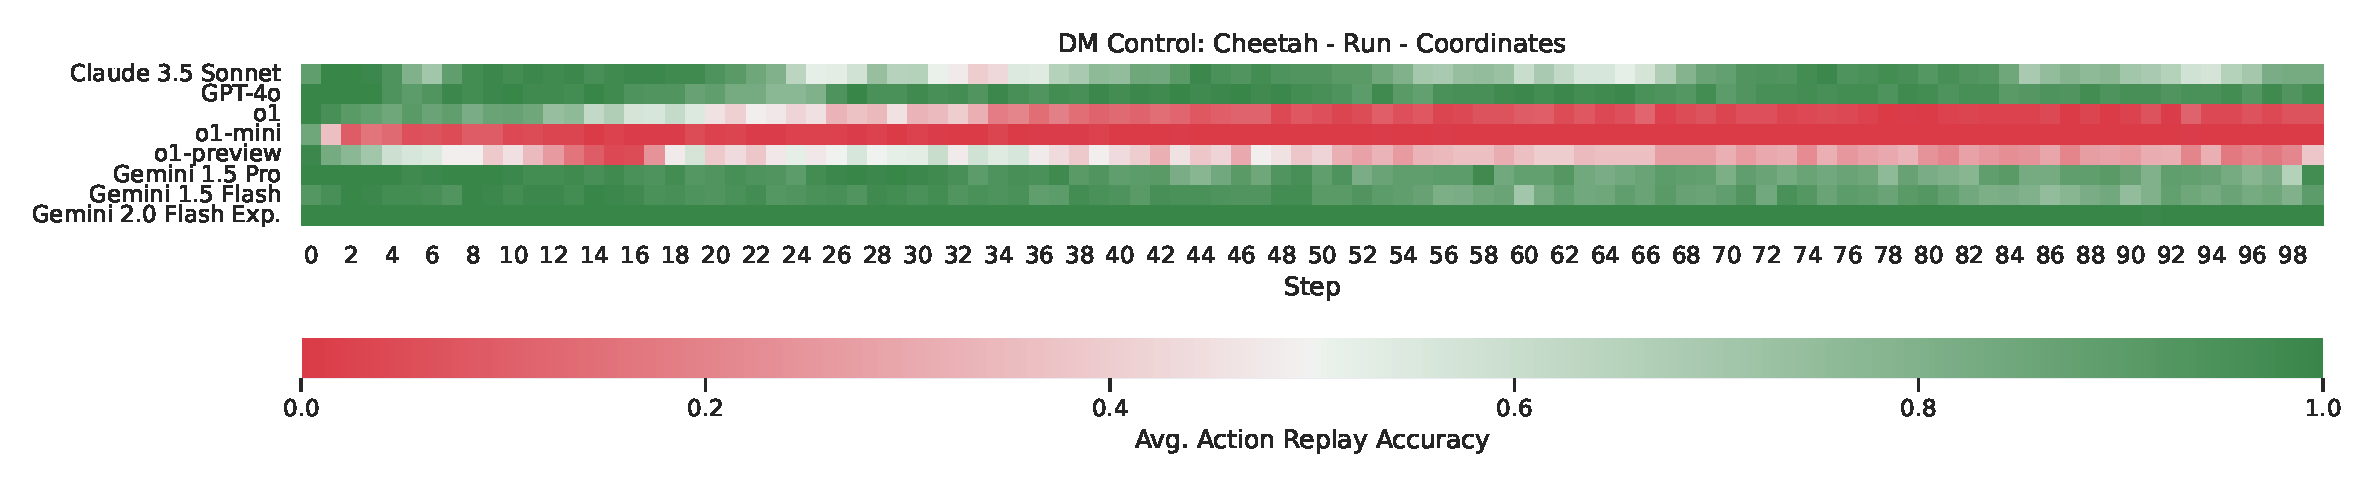
\includegraphics[width=\textwidth]{figures/dm_control_cheetah_run_dict_replay.eps}
    \end{center}
    \caption{
        Replaying the demonstration episode for the cheetah run task from the DM Control suite (with coordinate observations).
        The color visualizes the models' average accuracy when attempting to replay the action for a given step.
        \gpt{}, \flash{}, and \pro{} generally perform well.
        In contrast, \mini{} and \preview{} significantly struggle with this task.
        \claude{} shows patches of slightly poorer performance around steps $32$, $64$, and $96$, but performs well otherwise.
    }
    \label{fig:replay-dm-control}
\end{figure}

\begin{figure}
    \begin{subfigure}[t]{0.5\textwidth}
        \begin{center}
            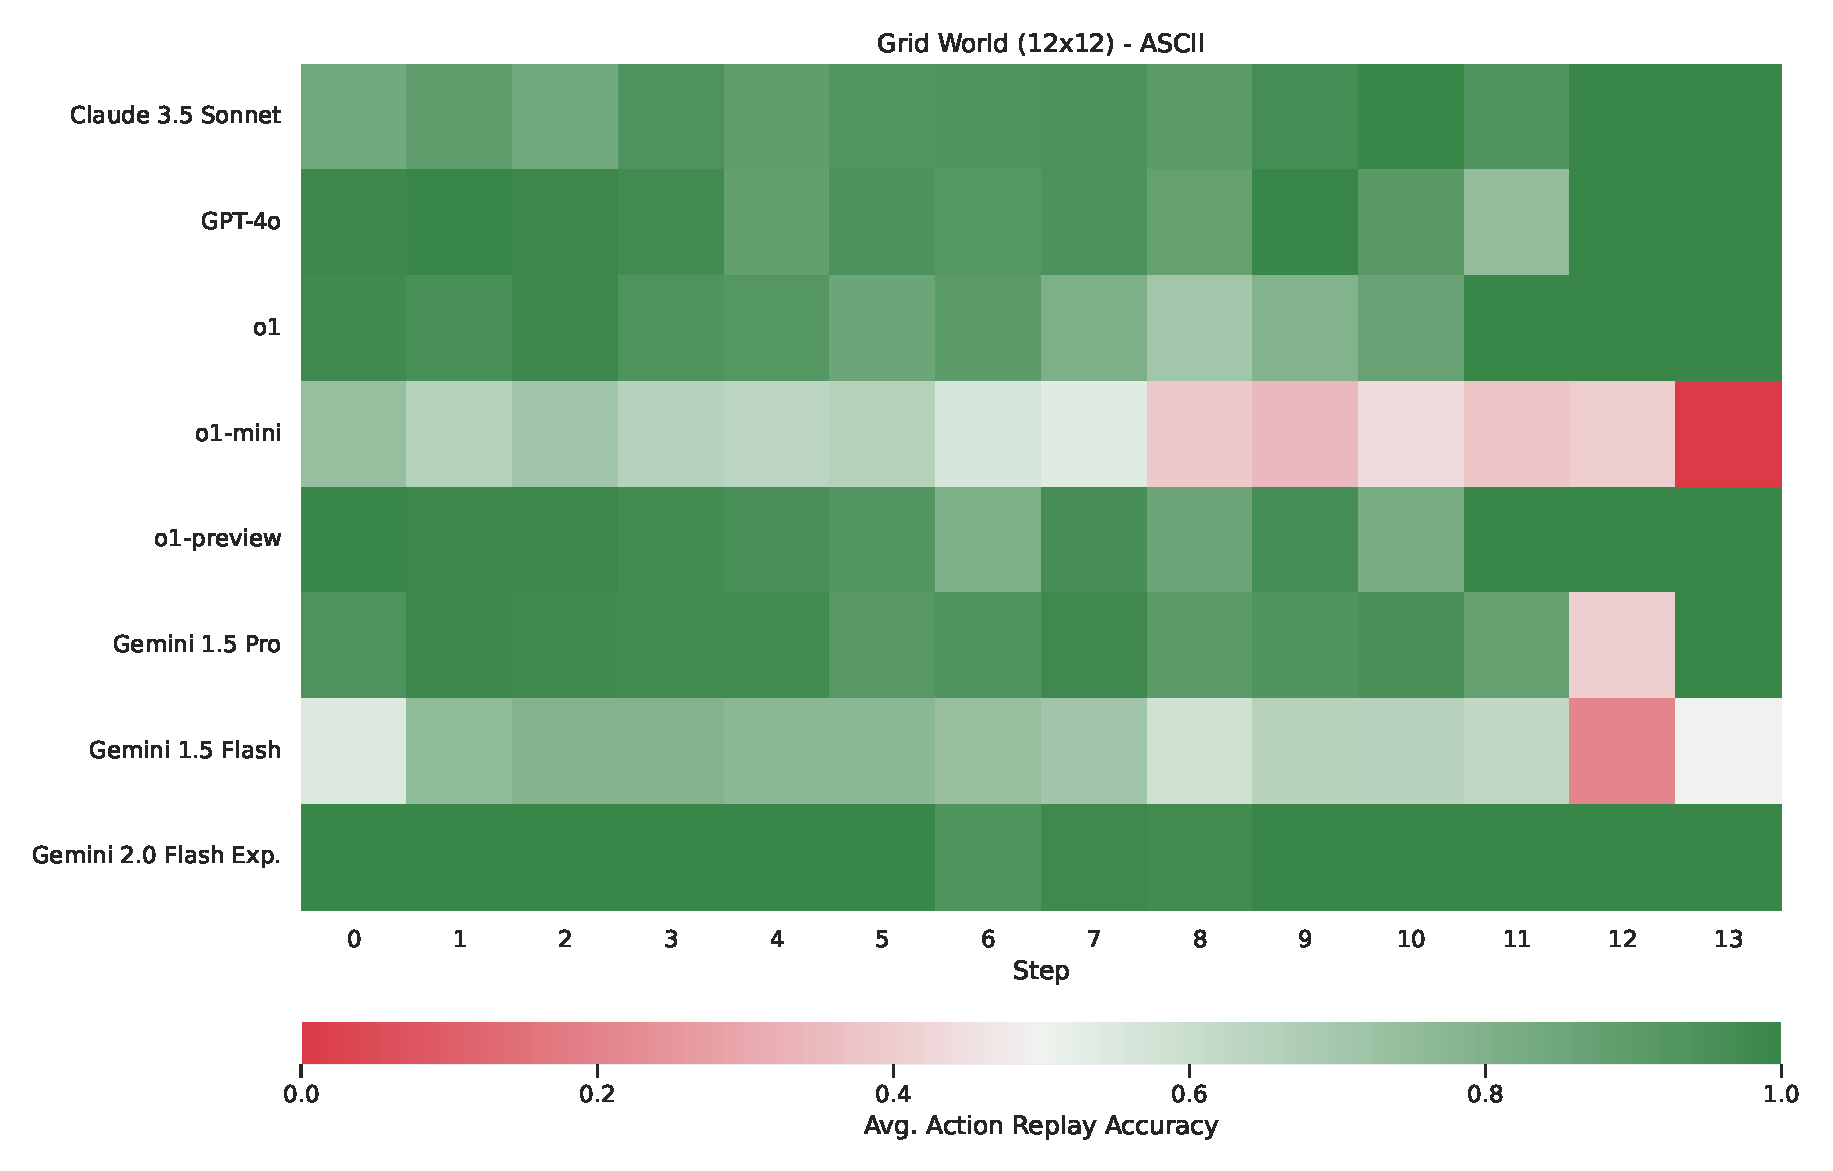
\includegraphics[width=\textwidth]{figures/grid_world_12x12_txt_replay.eps}
        \end{center}
       \caption{ASCII observations}
    \end{subfigure}
    \begin{subfigure}[t]{0.5\textwidth}
        \begin{center}
            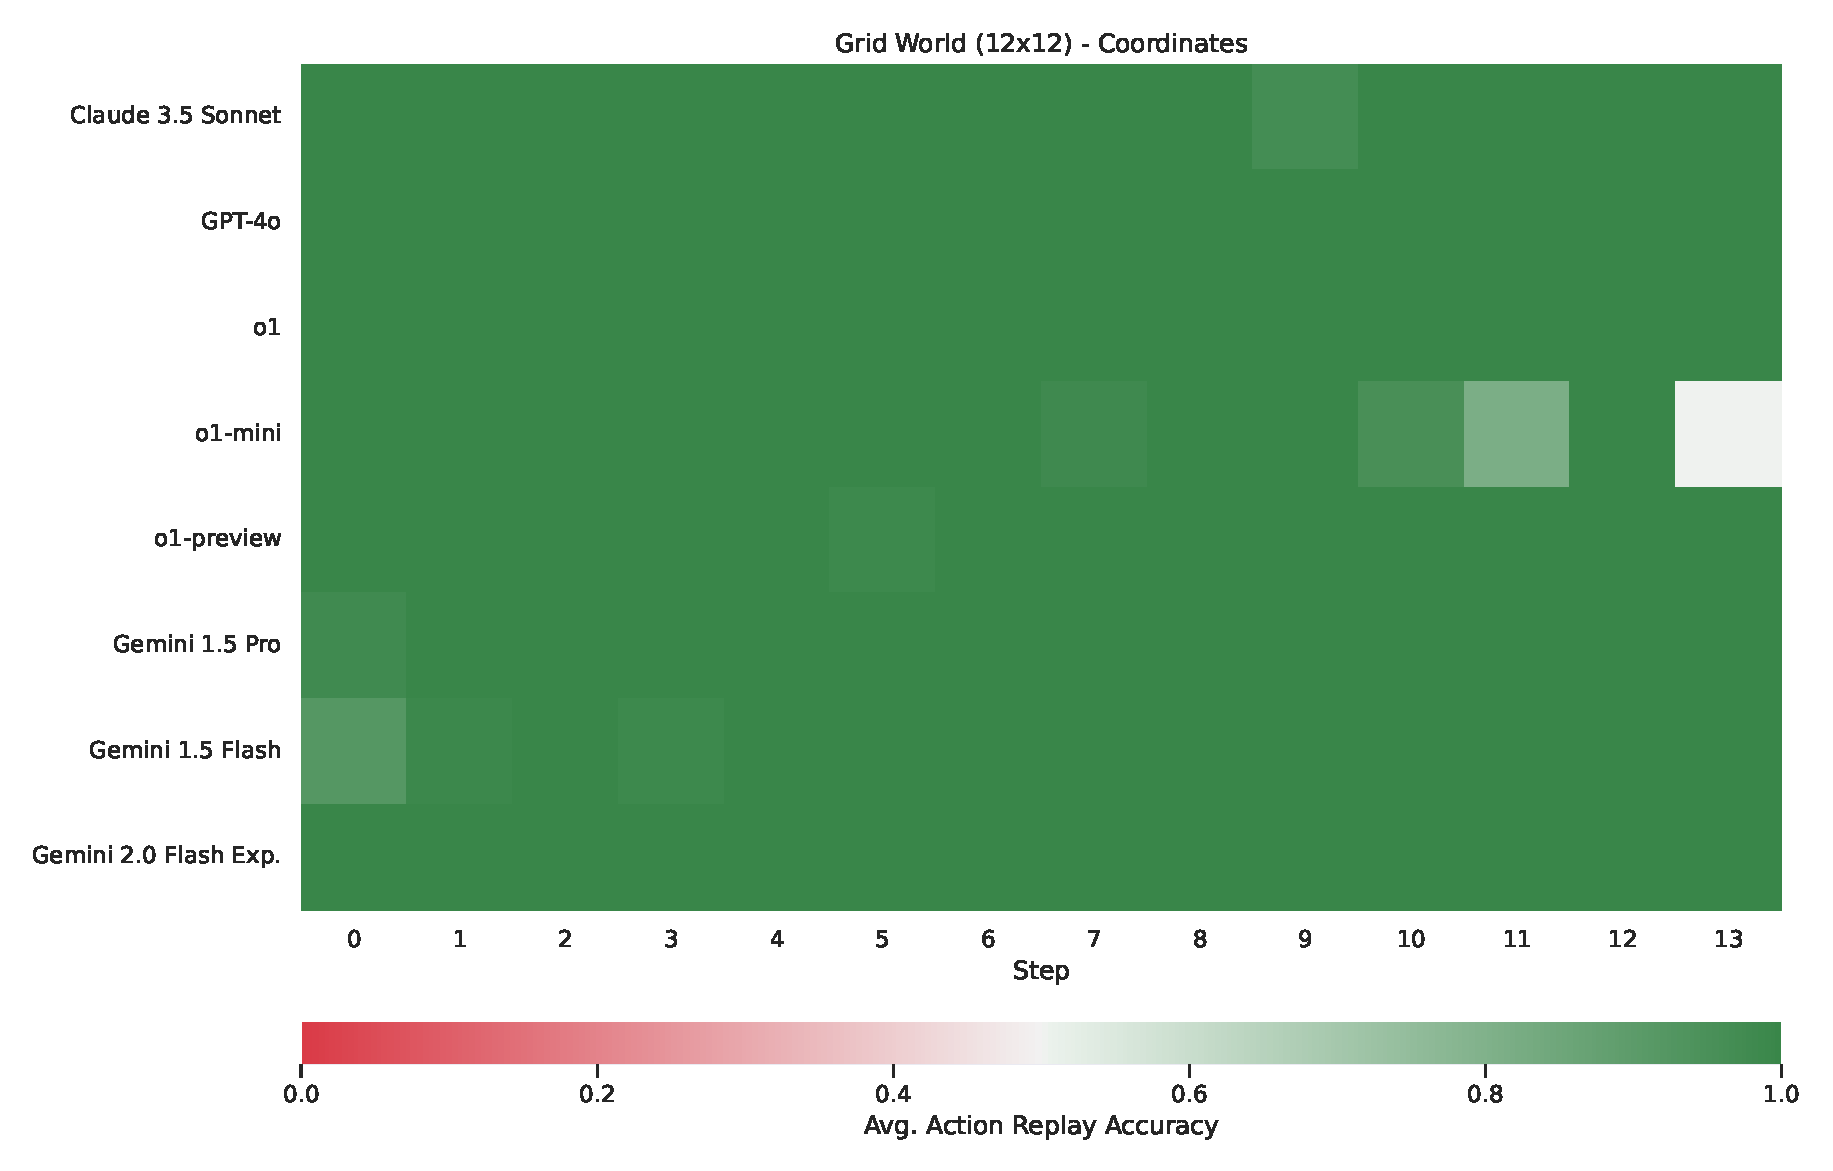
\includegraphics[width=\textwidth]{figures/grid_world_12x12_coords_replay.eps}
        \end{center}
        \caption{Coordinate observations}
    \end{subfigure}
    \par\bigskip
    \begin{subfigure}[t]{0.5\textwidth}
        \begin{center}
            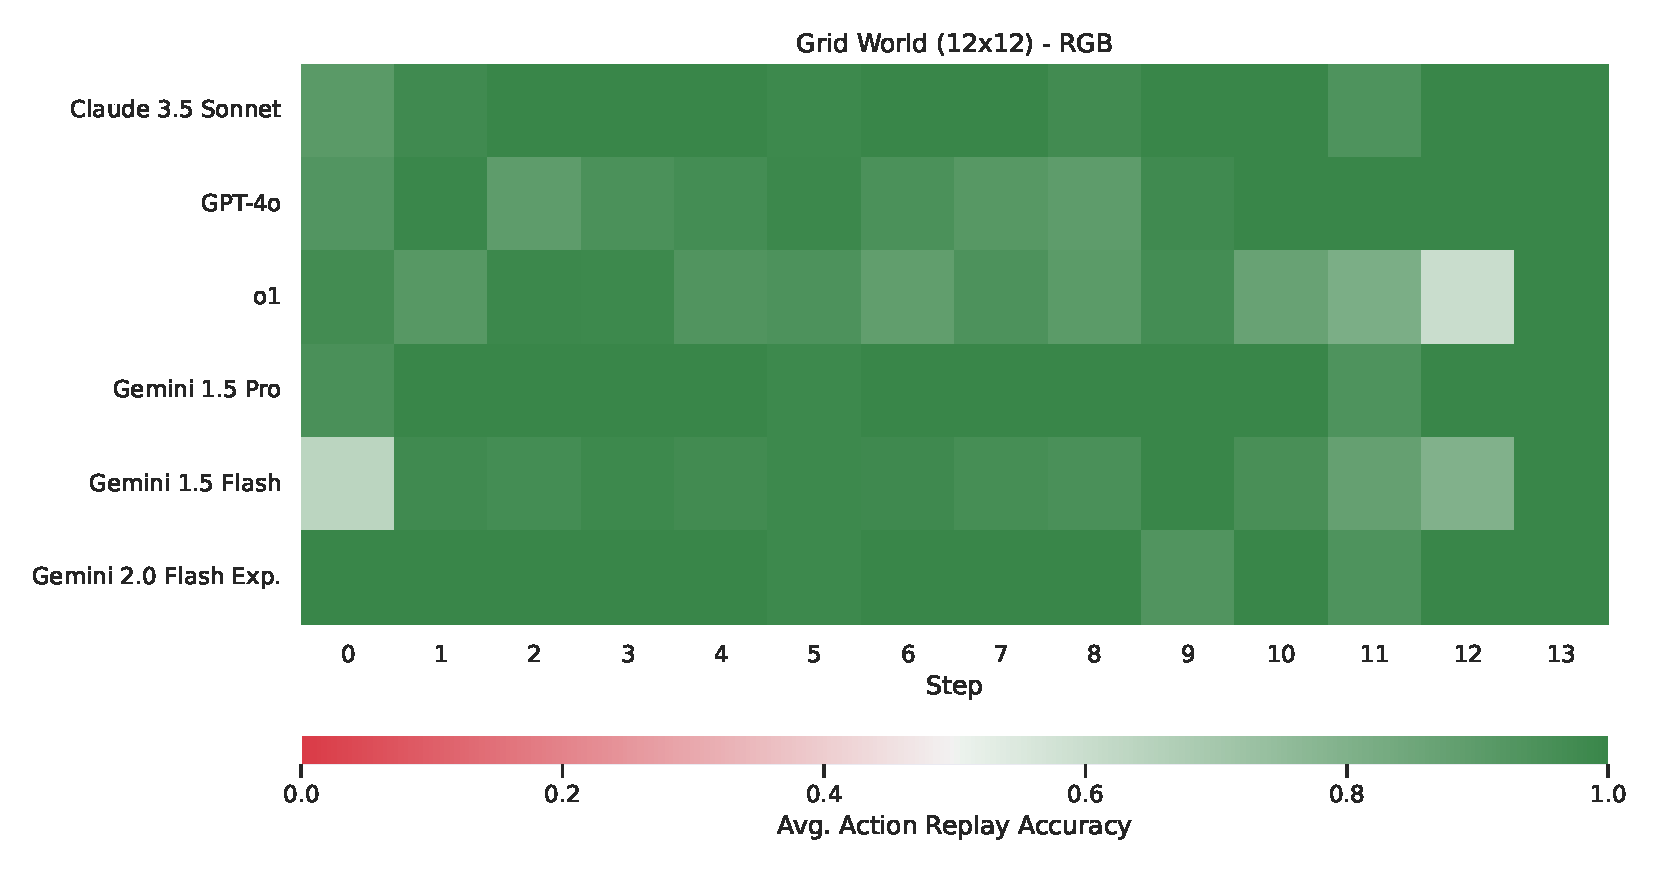
\includegraphics[width=\textwidth]{figures/grid_world_12x12_rgb_replay.eps}
        \end{center}
        \caption{RGB observations}
    \end{subfigure}
    \caption{
        Replaying the demonstration episode for the all observation types from our grid world navigation task.
        The color visualizes the models' average accuracy when attempting to replay the action for a given step.
        All models generally perform well across all observation types, except for \mini{} on ASCII observations.
        Moreover, the Gemini 1.5 models struggle on step $12$ with ASCII observations, and \mini{} struggles with the last step for coordinate observations.
        Note that \mini{} and \preview{} are text-only models and, therefore, cannot process RGB observations.
    }
    \label{fig:replay-grid-world}
\end{figure}

\begin{figure}
    \null\hfill
    \begin{subfigure}[t]{0.25\textwidth}
        \begin{center}
            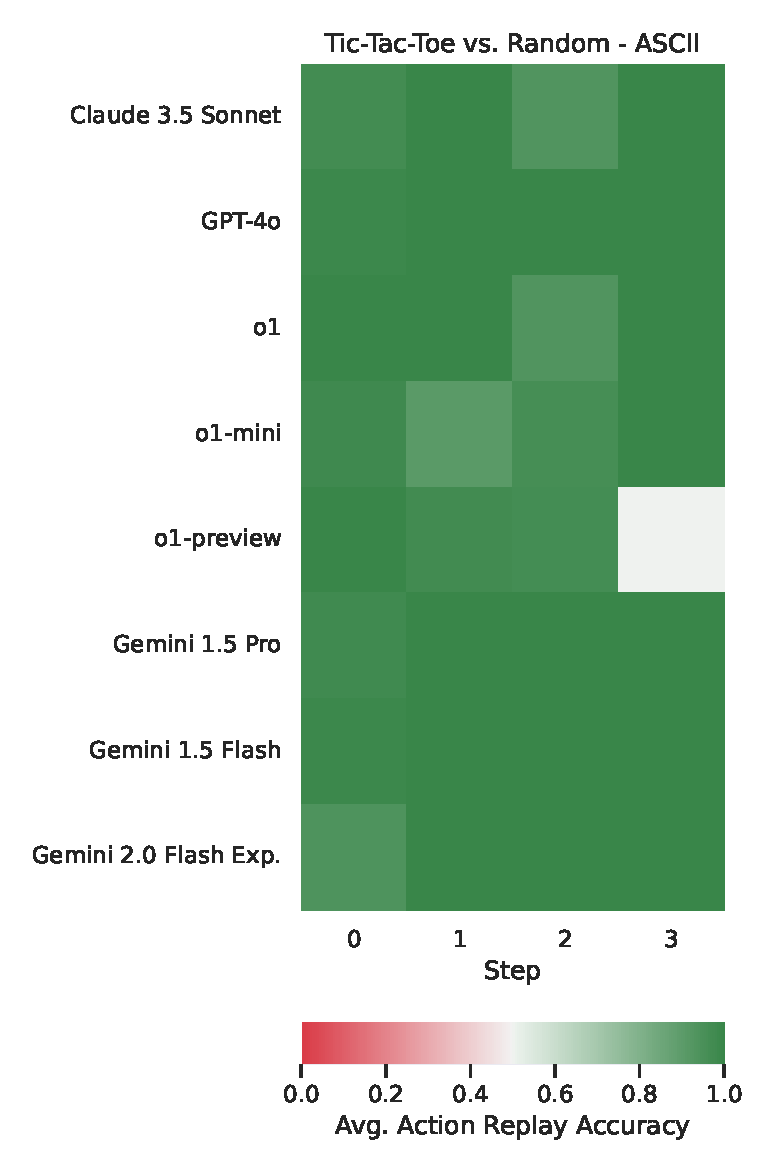
\includegraphics[width=\textwidth]{figures/tic_tac_toe_txt_replay.eps}
        \end{center}
        \caption{ASCII observations}
    \end{subfigure}
    \hfill
    \begin{subfigure}[t]{0.25\textwidth}
        \begin{center}
            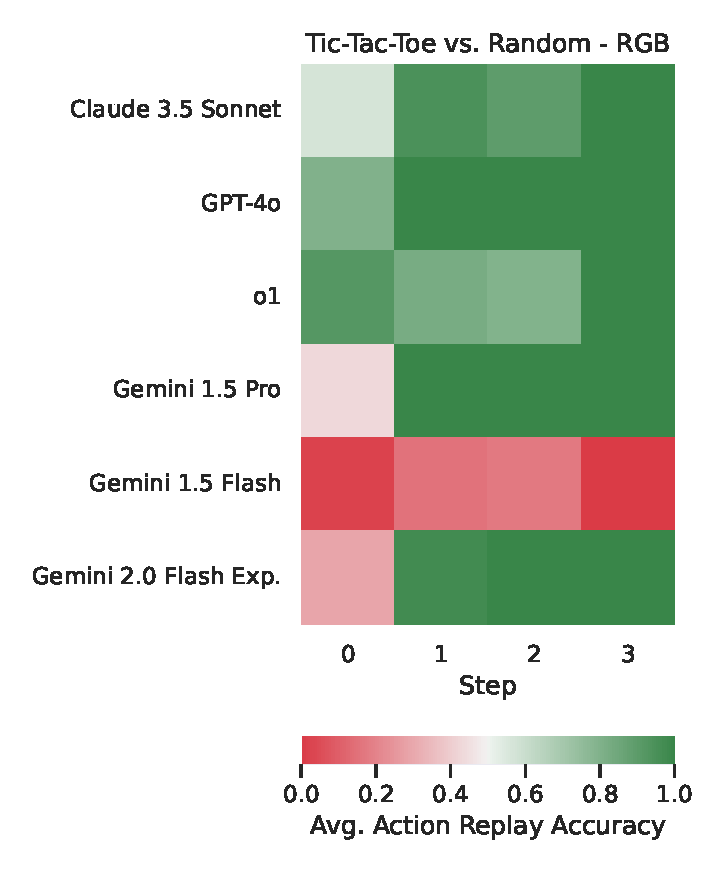
\includegraphics[width=\textwidth]{figures/tic_tac_toe_png_replay.eps}
        \end{center}
        \caption{RGB observations}
    \end{subfigure}
    \hfill\null
    \caption{
        Replaying the demonstration episode for the all observation types from our tic-tac-toe environment.
        The color visualizes the models' average accuracy when attempting to replay the action for a given step.
        All models generally perform well across all observation types except for \flash{} on RGB images, where it fails completely.
        \claude{} and \pro{} also struggle (to varying degrees) with the first step (step $0$) for RGB observations.
        Note that \mini{} and \preview{} are text-only models and, therefore, cannot process RGB image observations.
    }
    \label{fig:replay-tic-tac-toe}
\end{figure}


\begin{figure}
    \begin{subfigure}[t]{0.32\textwidth}
        \begin{center}
            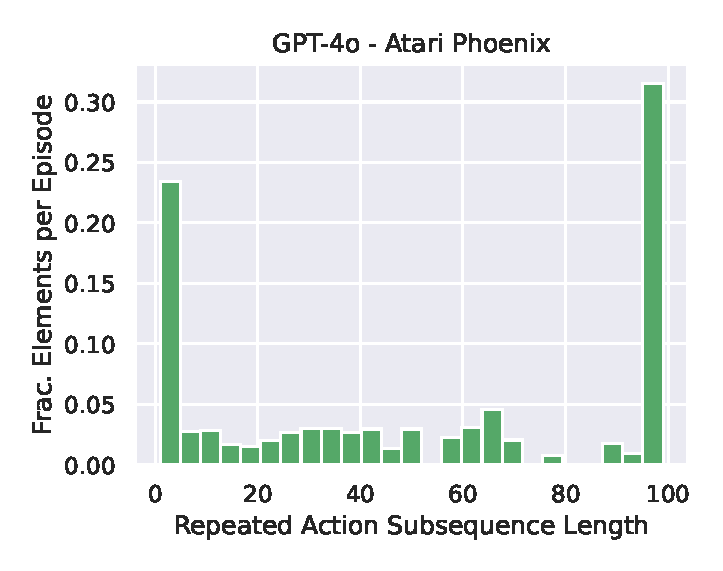
\includegraphics[width=\textwidth]{figures/atari_phoenix_gpt_4o_subsequences}
        \end{center}
       \caption{\gpt{}}
    \end{subfigure}
    \hfill
    \begin{subfigure}[t]{0.32\textwidth}
        \begin{center}
            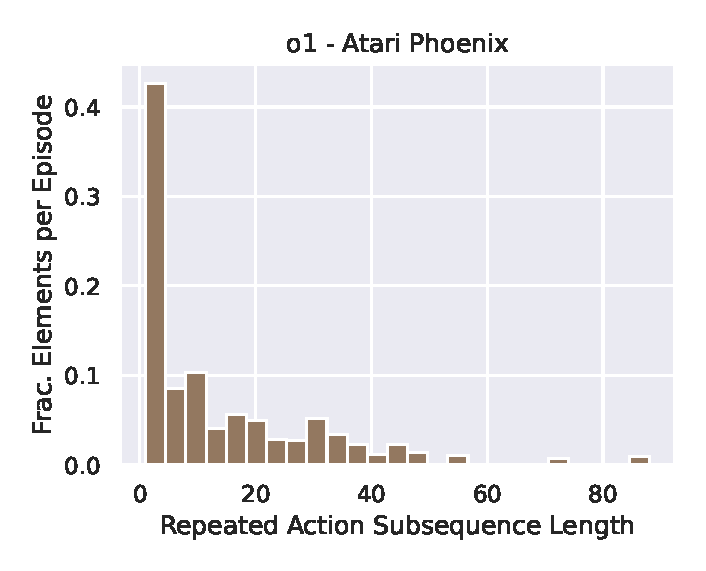
\includegraphics[width=\textwidth]{figures/atari_phoenix_o1_subsequences}
        \end{center}
       \caption{o1}
    \end{subfigure}
    
    \begin{subfigure}[t]{0.32\textwidth}
        \begin{center}
            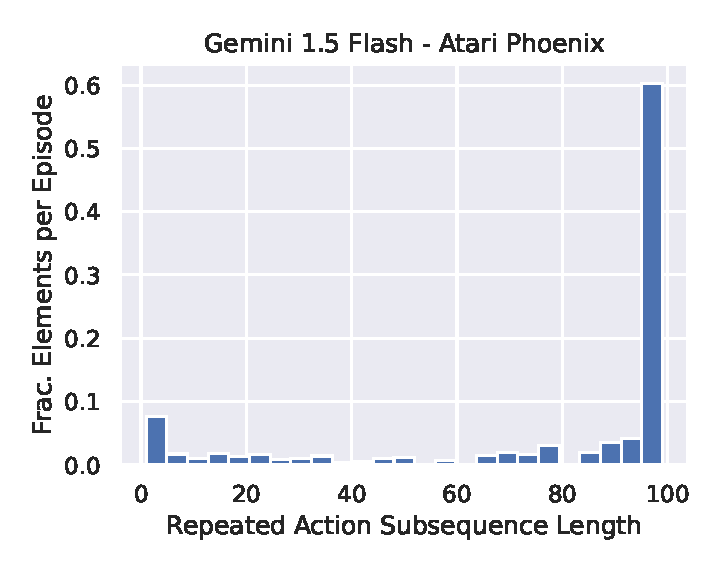
\includegraphics[width=\textwidth]{figures/atari_phoenix_gemini_1_5_flash_subsequences}
        \end{center}
        \caption{\flash{}}
    \end{subfigure}
    \hfill
    \begin{subfigure}[t]{0.32\textwidth}
        \begin{center}
            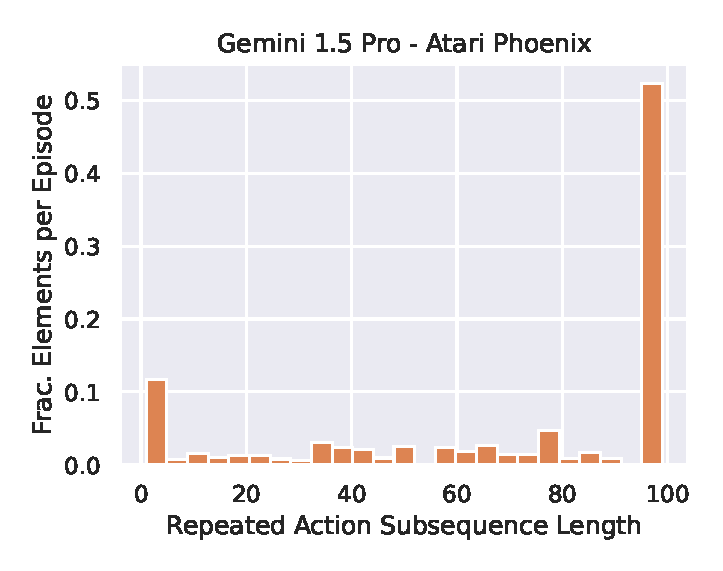
\includegraphics[width=\textwidth]{figures/atari_phoenix_gemini_1_5_pro_subsequences}
        \end{center}
        \caption{\pro{}}
    \end{subfigure}
    \hfill
    \begin{subfigure}[t]{0.32\textwidth}
        \begin{center}
            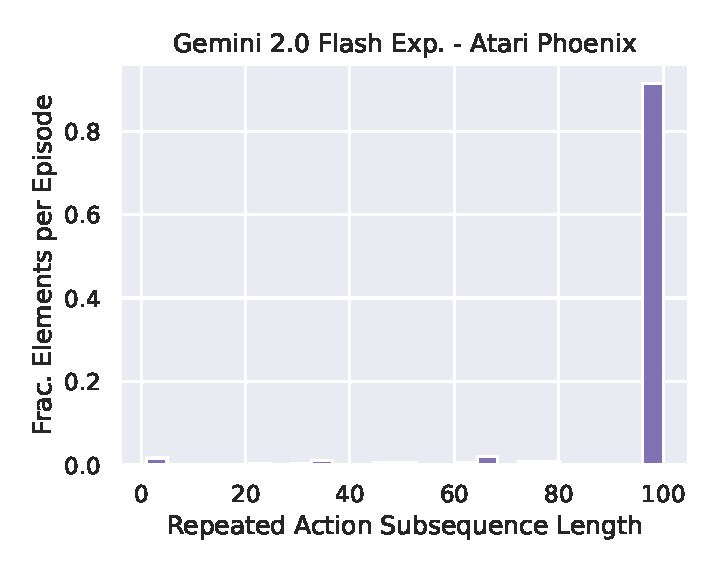
\includegraphics[width=\textwidth]{figures/atari_phoenix_gemini_2_0_flash_exp__subsequences}
        \end{center}
        \caption{\expflash{}}
    \end{subfigure}
    \caption{
        Fraction of elements per repeated action subsequence length in the Phoenix game from Atari $2600$ (without demonstration episodes).
        To compute these results, we partition each evaluation episode into segments consisting of the same action generated consecutively.
        The segment length is on the x-axis, and the height of each bar is the fraction of actions (out of the total number of actions) across all time steps in all evaluation episodes that fall into each segment length.
        All three models have many episodes (\eg more than $60$\% for \flash{}) where they repeat the same action throughout almost the entire episode.
        Accordingly, they fire very rarely and thus achieve a low score (\cf \cref{fig:atari-phoenix}), since, in the Phoenix game, in order to fire repeatedly, the firing button needs to be pressed and released repeatedly --- constantly holding it down (\ie repeating the previous action) only results in a single shot.
    }
    \label{fig:atari-subsequence-length}
\end{figure}

\subsection{Illegal Actions}
\label{app:additional-results:illegal-actions}

\begin{figure}
    \begin{center}
        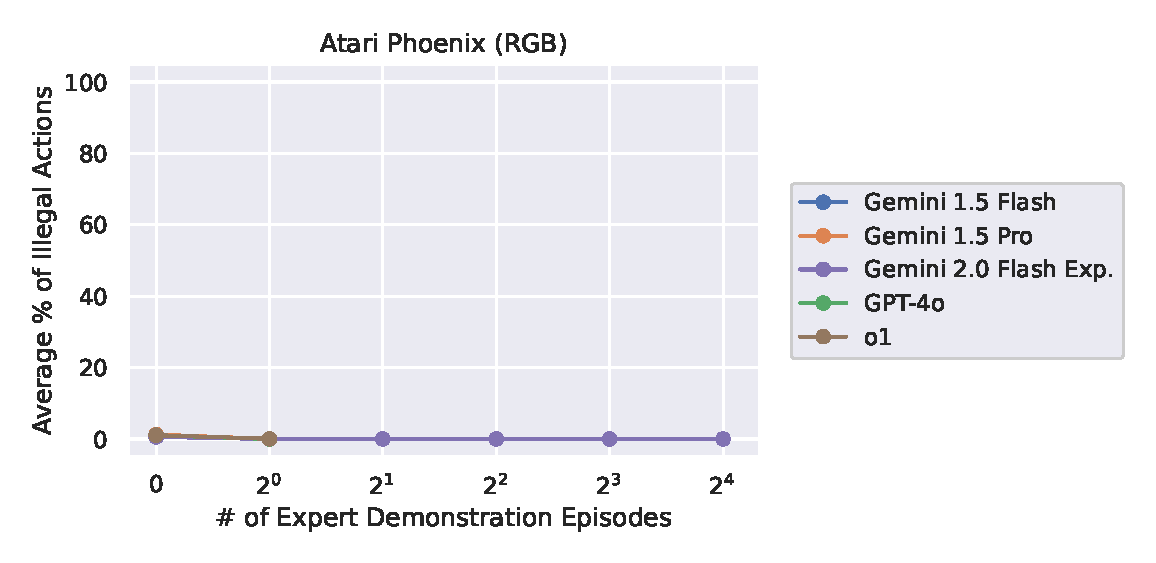
\includegraphics[width=0.5\textwidth]{figures/atari_phoenix_rgb_illegal_actions.eps}
    \end{center}
    \caption{
        Average percentage of illegal actions per episode over the number of expert demonstrations for the Phoenix game (RGB observations) from Atari 2600.
        All models mostly generate legal actions.
        Note that \mini{} and \preview{} are text-only and, thus, cannot process RGB observations.
    }
    \label{fig:atari-illegal-actions}
\end{figure}

As described in \cref{sec:methods:evaluation-protocol}, we do not terminate the evaluation episode early if a model does not produce a valid action (except on the crossword task) but instead randomly sample one of the actions that are legal in the current state and continue the evaluation with the observation produced by that action.
To differentiate illegal actions from acting randomly (over legal actions), we compute how often models actually propose an illegal action and visualize the percentage of illegal actions per episode over the number of expert demonstrations in \cref{fig:atari-illegal-actions,fig:chess-illegal-actions,fig:crossword-illegal-actions,fig:dm-control-illegal-actions,fig:grid-world-illegal-actions,fig:tic-tac-toe-illegal-actions} (analogous to \cref{fig:atari-phoenix,fig:chess,fig:crossword,fig:dm-control,fig:grid-world,fig:tic-tac-toe}).
Note that, since we perform an ablation over \emph{showing the legal moves in the prompt} (see \cref{app:additional-results:ablations}), in theory, all models could have the necessary information to sample a legal action at all times (whether we actually show this or not in our main experiments depends on whether it improves model performance in the ablations).
Nevertheless, we observe that models do produce illegal actions actions across most environments.
For example, on the grid world navigation task with coordinate observations \preview{} produces almost $100$\% illegal actions with $2$ or more expert demonstrations in the context.
Interestingly, the ability to produce legal actions also depends on the observation type: For tic-tac-toe, all models mostly produce legal actions with ASCII observations, but the Gemini 1.5 models generate up to $\sim60$\% illegal actions for RGB observations from the same environment.

\begin{figure}
    \begin{subfigure}[t]{0.5\textwidth}
        \begin{center}
            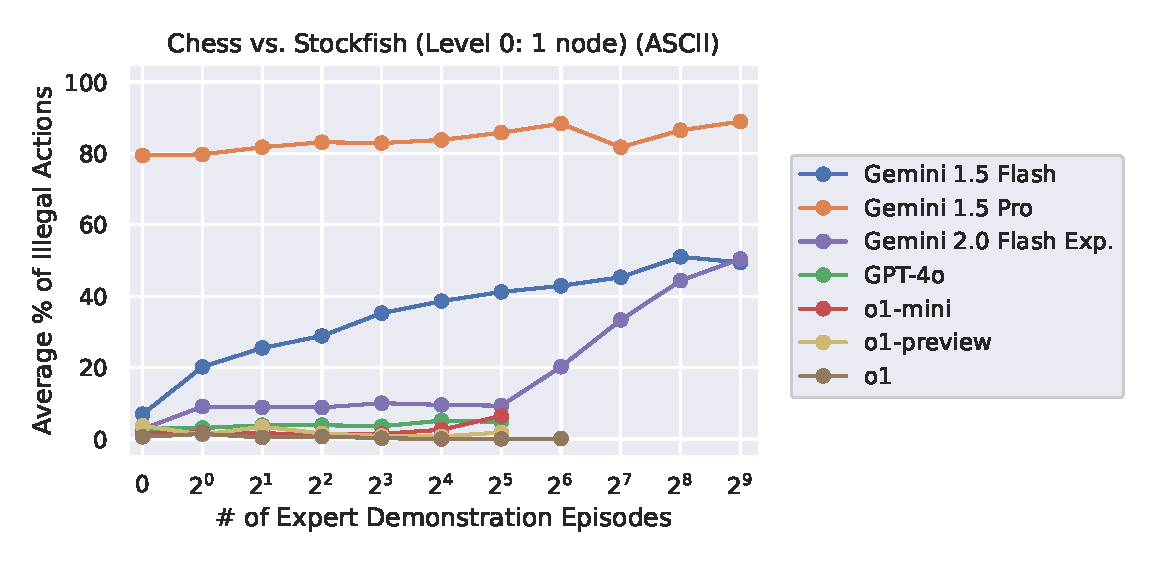
\includegraphics[width=\textwidth]{figures/chess_txt_illegal_actions.eps}
        \end{center}
        \caption{ASCII observations}
    \end{subfigure}
    \begin{subfigure}[t]{0.5\textwidth}
        \begin{center}
            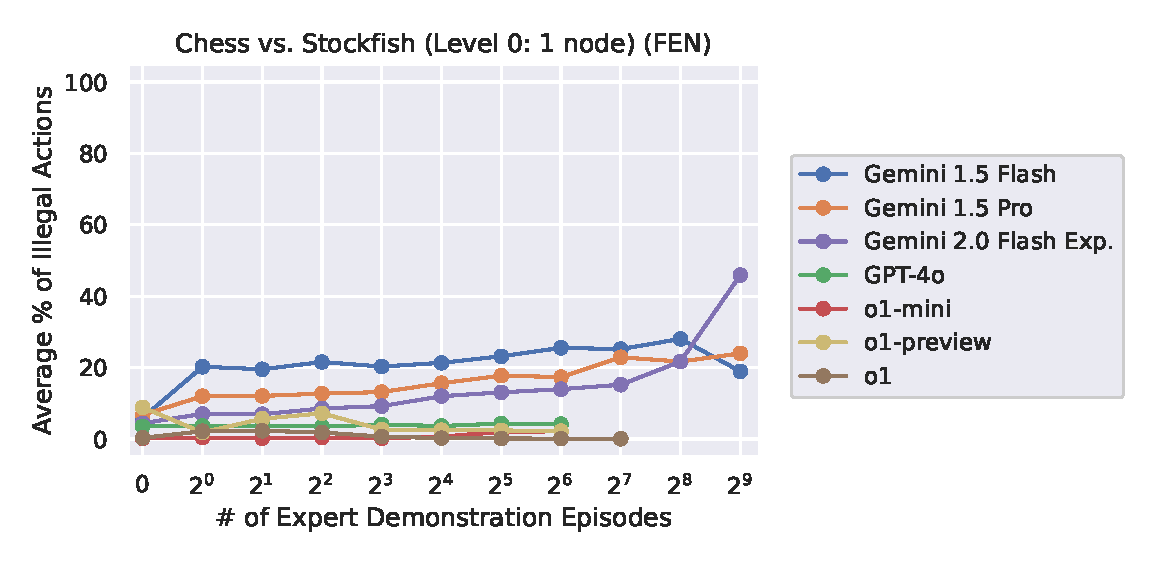
\includegraphics[width=\textwidth]{figures/chess_fen_illegal_actions.eps}
        \end{center}
        \caption{FEN observations}
    \end{subfigure}
    \par\bigskip
    \begin{subfigure}[t]{0.5\textwidth}
        \begin{center}
            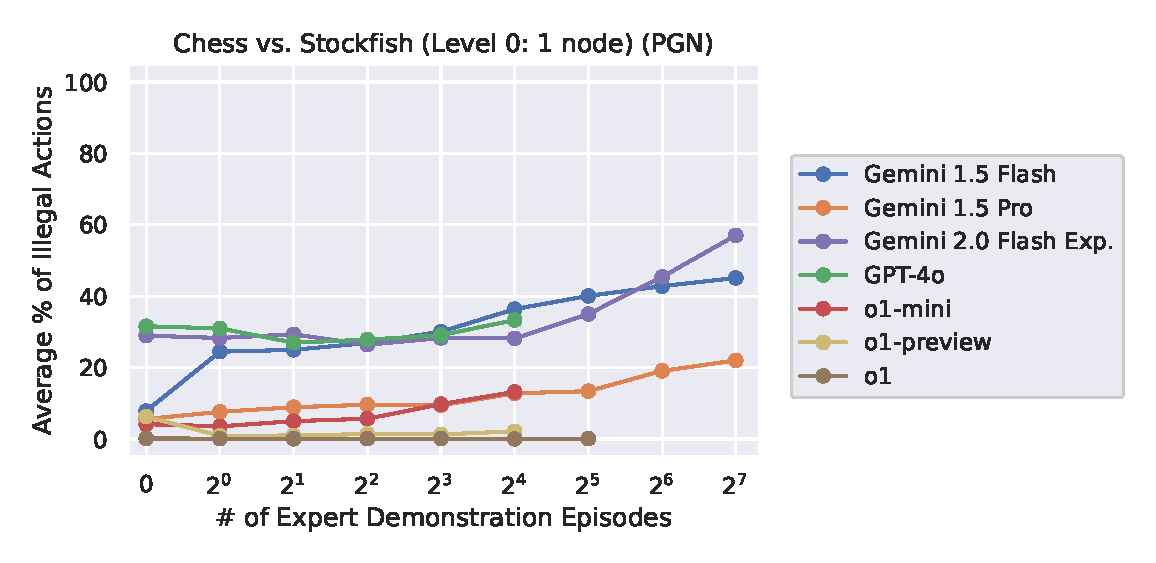
\includegraphics[width=\textwidth]{figures/chess_pgn_illegal_actions.eps}
        \end{center}
        \caption{PGN observations}
    \end{subfigure}
    \begin{subfigure}[t]{0.5\textwidth}
        \begin{center}
            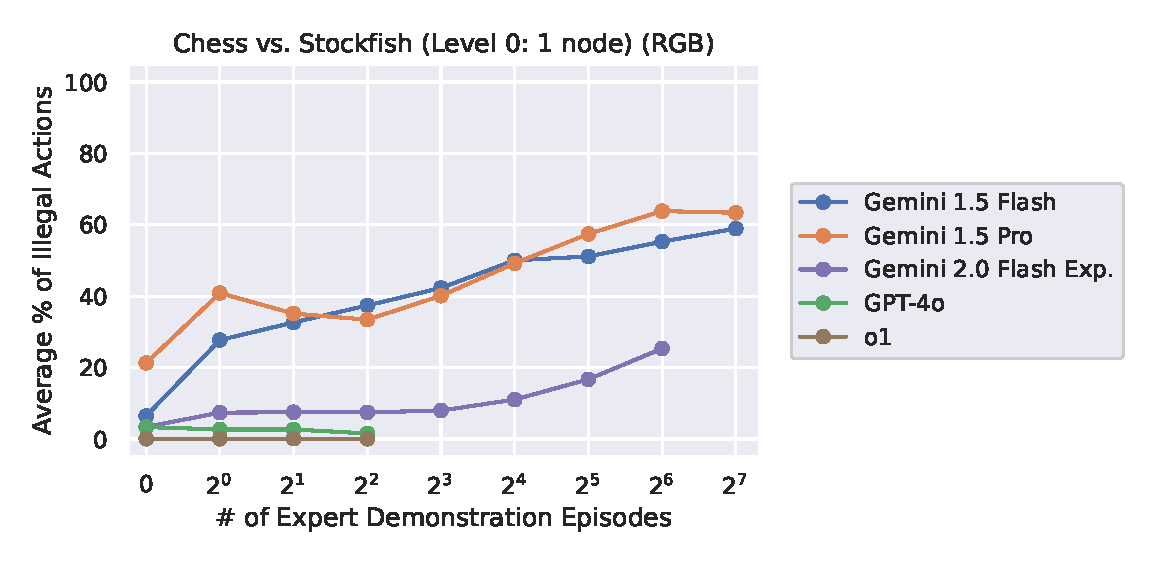
\includegraphics[width=\textwidth]{figures/chess_png_illegal_actions.eps}
        \end{center}
        \caption{RGB observations}
    \end{subfigure}
    \caption{
        Average percentage of illegal actions per episode over the number of expert demonstrations for all state representation formats from our chess environment.
        \gpt{}, \mini{}, and \preview{} rarely generate illegal actions (except for \gpt{} with PGN observations).
        In contrast, the Gemini 1.5 models consistently struggle to generate legal actions across all state representation formats and with higher rates of illegal actions with increasing numbers of expert demonstrations in the context.
        Note that \mini{} and \preview{} are text-only models and therefore cannot process RGB image observations.
    }
    \label{fig:chess-illegal-actions}
\end{figure}

\begin{figure}
    \begin{minipage}{0.475\textwidth}
            \begin{center}
                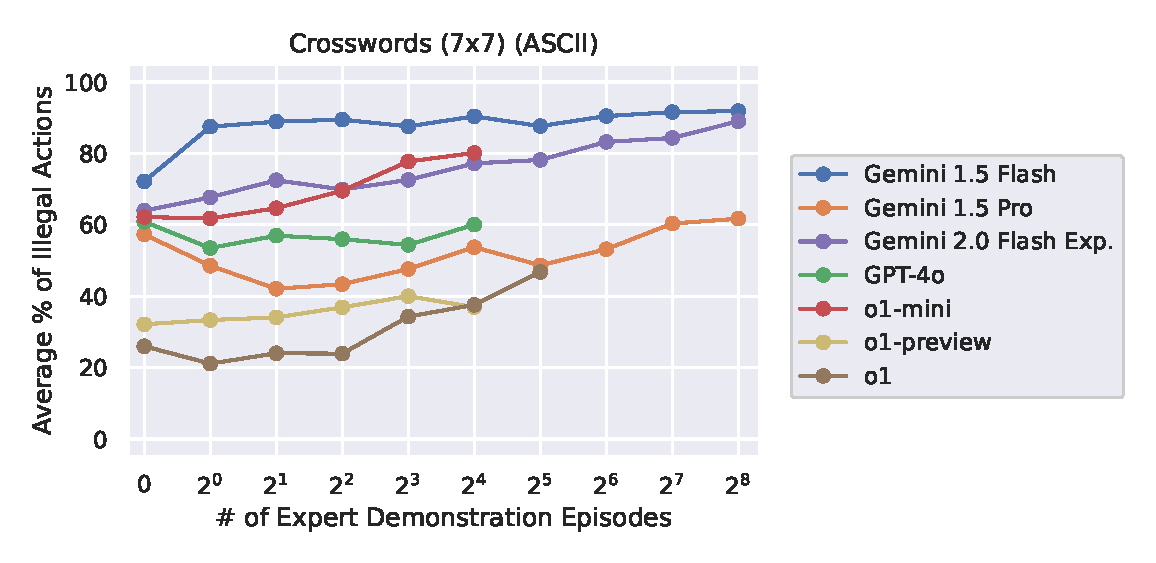
\includegraphics[width=\textwidth]{figures/crossword_txt_illegal_actions.eps}
            \end{center}
            \captionof{figure}{
                Average percentage of illegal actions per episode over the number of expert demonstrations for our crossword environment with ASCII observations.
                All models produce a high percentage of illegal actions (between $\sim40$\% and $\sim90$\% of all the actions in an episode).
            }
            \label{fig:crossword-illegal-actions}
    \end{minipage}
    \hfill
    \begin{minipage}{0.475\textwidth}
            \begin{center}
                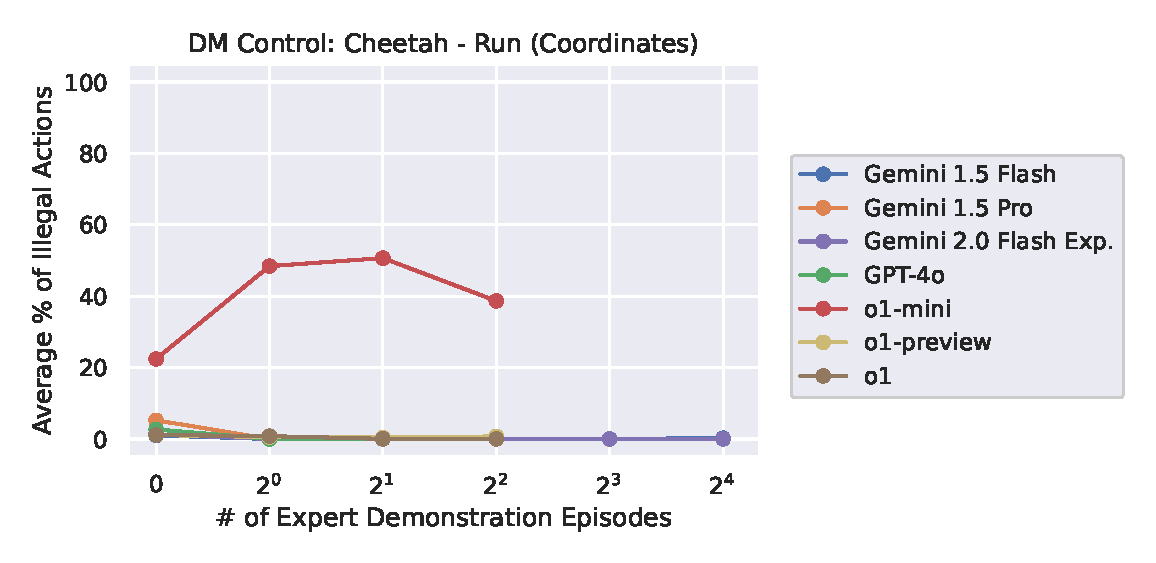
\includegraphics[width=\textwidth]{figures/dm_control_cheetah_run_dict_illegal_actions.eps}
            \end{center}
            \captionof{figure}{
                Average percentage of illegal actions per episode over the number of expert demonstrations for the cheetah run task from the DM Control suite with coordinate observations.
                All models, except \mini{}, consistently produce mostly legal actions.
            }
            \label{fig:dm-control-illegal-actions}
    \end{minipage}
\end{figure}

\begin{figure}
    \begin{subfigure}[t]{0.5\textwidth}
        \begin{center}
            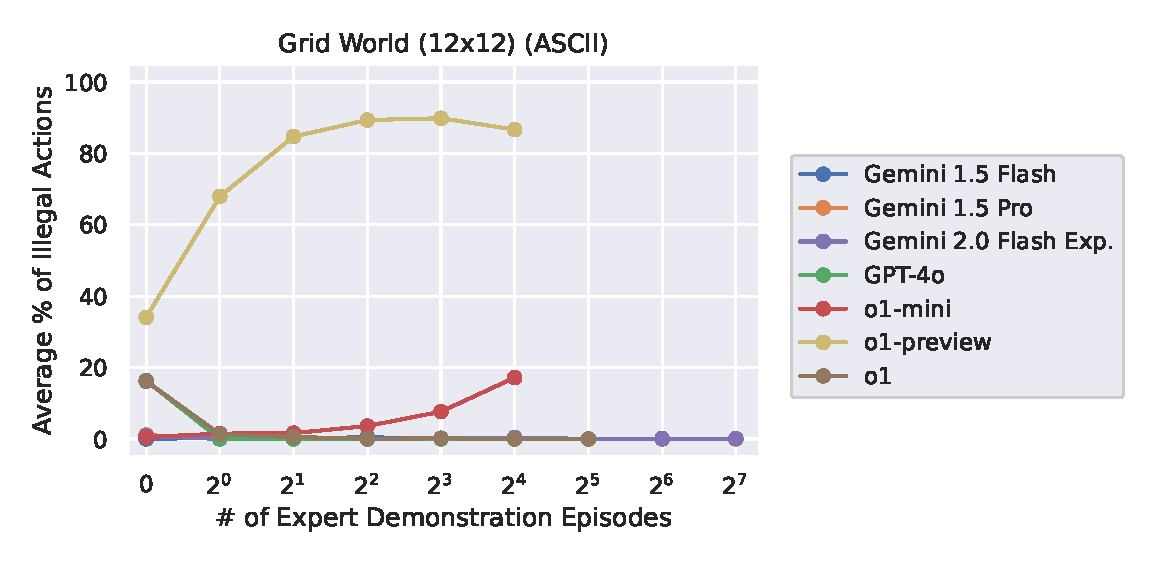
\includegraphics[width=\textwidth]{figures/grid_world_12x12_txt_illegal_actions.eps}
        \end{center}
        \caption{ASCII observations}
    \end{subfigure}
    \begin{subfigure}[t]{0.5\textwidth}
        \begin{center}
            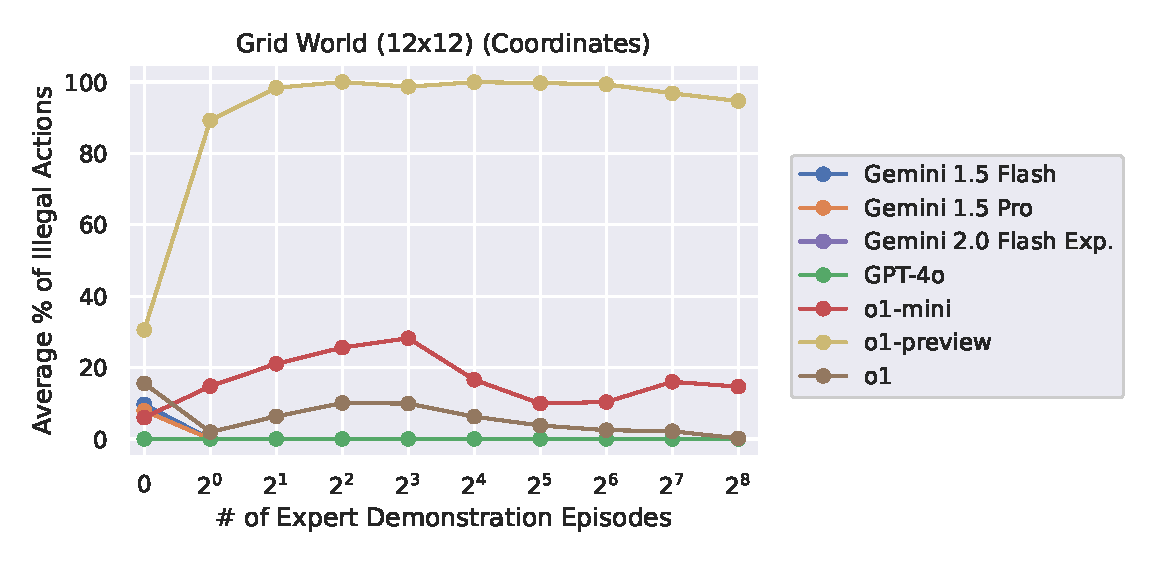
\includegraphics[width=\textwidth]{figures/grid_world_12x12_coords_illegal_actions.eps}
        \end{center}
        \caption{Coordinate observations}
    \end{subfigure}
    \par\bigskip
    \begin{subfigure}[t]{0.5\textwidth}
        \begin{center}
            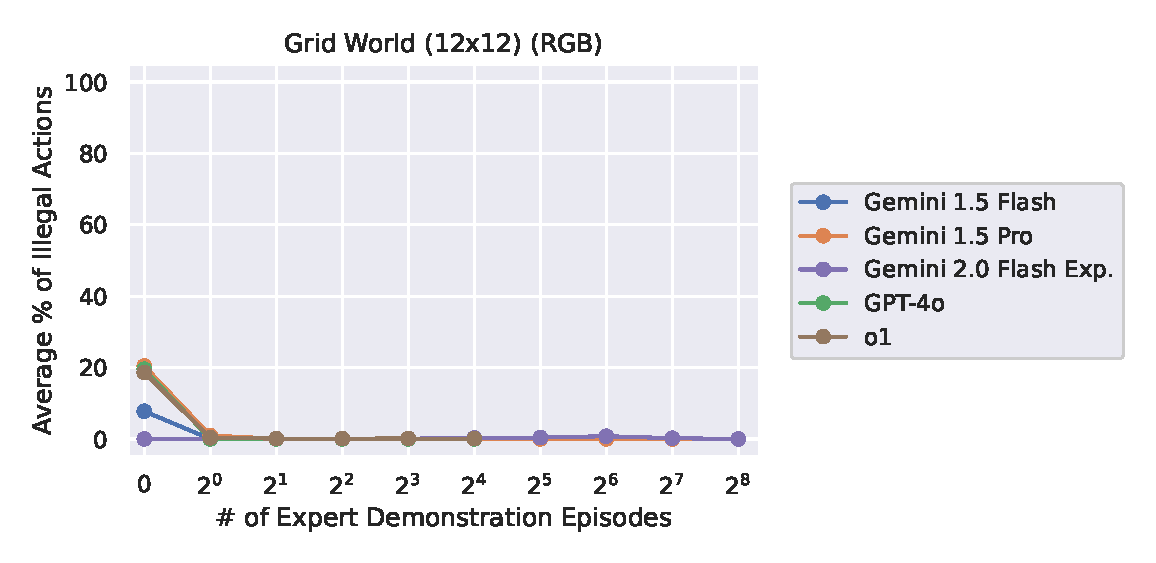
\includegraphics[width=\textwidth]{figures/grid_world_12x12_rgb_illegal_actions.eps}
        \end{center}
        \caption{RGB observations}
    \end{subfigure}
    \caption{
        Average percentage of illegal actions per episode over the number of expert demonstrations for all state representation formats form our grid world navigation task.
        The o1 models increasingly struggle to produce legal actions with increasing numbers of expert demonstrations in the context, with \preview{} having a very high percentage of illegal actions.
        In contrast, \gpt{}, \flash{}, and \pro{} consistently produce legal actions.
        Note that \mini{} and \preview{} are text-only models and therefore cannot process RGB image observations.
    }
    \label{fig:grid-world-illegal-actions}
\end{figure}

\begin{figure}
    \begin{subfigure}[t]{0.5\textwidth}
        \begin{center}
            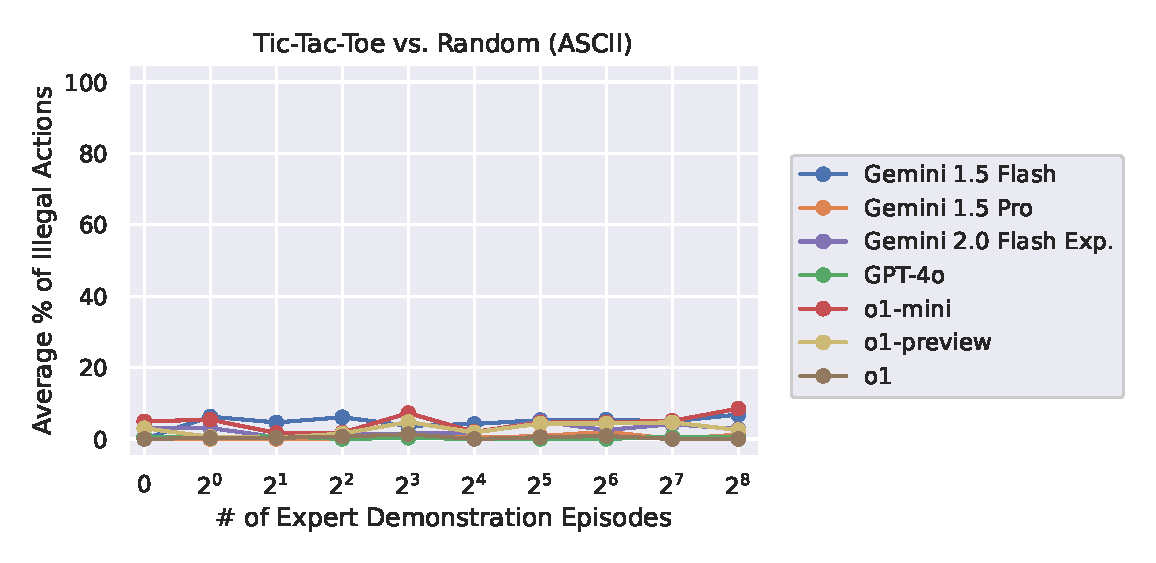
\includegraphics[width=\textwidth]{figures/tic_tac_toe_txt_illegal_actions.eps}
        \end{center}
        \caption{ASCII observations}
    \end{subfigure}
    \begin{subfigure}[t]{0.5\textwidth}
        \begin{center}
            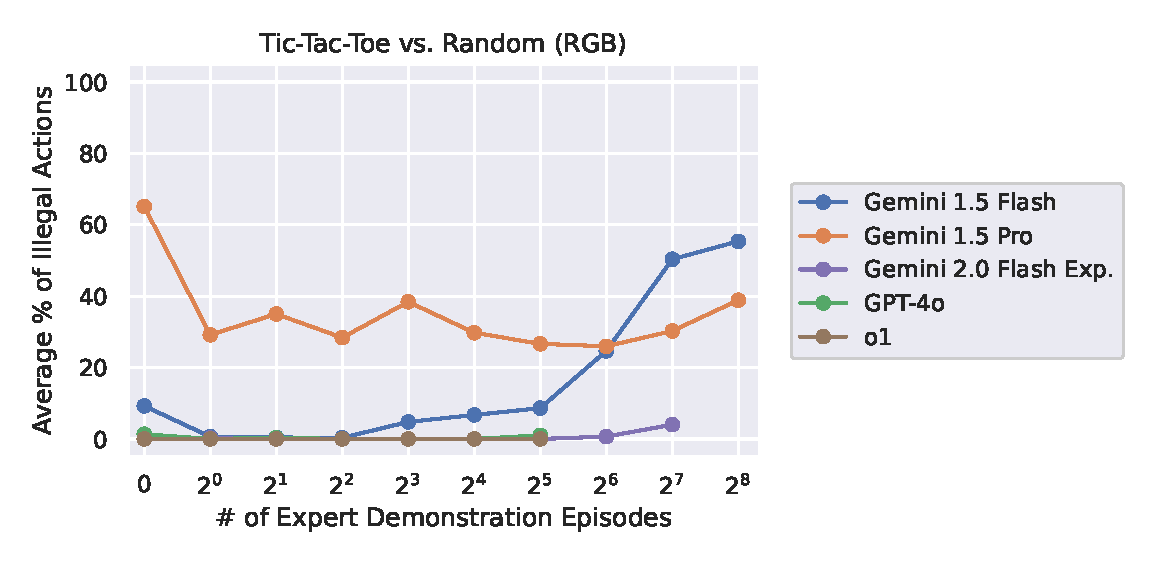
\includegraphics[width=\textwidth]{figures/tic_tac_toe_png_illegal_actions.eps}
        \end{center}
        \caption{RGB observations.}
    \end{subfigure}
    \caption{
        Average percentage of illegal actions per episode over the number of expert demonstrations for all state representation formats from our tic-tac-toe environment.
        With ASCII observations, all models mostly produce legal actions.
        In contrast, for RGB image observations, the Gemini 1.5 models struggle to produce legal actions (\pro{} independently of the number of expert demonstrations and \flash{} increasingly with the number of expert demonstrations).
        Note that \mini{} and \preview{} are text-only models and therefore cannot process RGB image observations.
    }
    \label{fig:tic-tac-toe-illegal-actions}
\end{figure}


\subsection{Hyperparameter Ablations}
\label{app:additional-results:ablations}

As mentioned in \cref{sec:results}, we ablate the use of chain-of-though prompting~\citep{wei2022chain} and whether or not to include the list of actions that is legal given the current observation in the prompt for each model-task combination since we want to report the best-possible performance the models can attain on our benchmark.
For completeness, we present all the ablation results in  \cref{tab:atari-ablation,tab:chess-ablation-anthropic,tab:chess-ablation-gemini,tab:chess-ablation-openai,tab:crossword-ablation,tab:dm-control-ablation,tab:grid-world-ablation-anthropic,tab:grid-world-ablation-gemini,tab:grid-world-ablation-openai,tab:tic-tac-toe-ablation}.
We highlight the best score for each model-observation pair in bold and use the corresponding hyperparameter combination for our sweeps over the number of expert demonstration episodes in \cref{sec:results:in-context-imitation-learning}.

\begin{table}
    \caption{
        Ablating the use of chain-of-thought prompting and whether or not to show legal actions in the prompt for the Phoenix game from Atari 2600.
        For this task, all models perform best without legal actions and without chain-of-thought.
    }
    \begin{center}
        \resizebox{0.55\textwidth}{!}{\begin{tabular}{@{}llllr@{}}
    \toprule
    \textbf{Model}                                                      & \textbf{Observation}      & \textbf{Legal Actions}    & \textbf{Chain-of-Thought} & \textbf{Average Score} \\
    \midrule
    \multirow[c]{4}{*}{Gemini 1.5 Flash}                                & \multirow[c]{4}{*}{RGB}   & \multirow[c]{2}{*}{False} & False                     & \textbf{42.83} \\
                                                                        &                           &                           & True                      & 6.16 \\
                                                                        &                           & \multirow[c]{2}{*}{True}  & False                     & 8.07 \\
                                                                        &                           &                           & True                      & 6.46 \\
    \midrule                                                                                                                                                   
    \multirow[c]{4}{*}{Gemini 1.5 Pro}                                  & \multirow[c]{4}{*}{RGB}   & \multirow[c]{2}{*}{False} & False                     & \textbf{21.86} \\
                                                                        &                           &                           & True                      & 8.68 \\
                                                                        &                           & \multirow[c]{2}{*}{True}  & False                     & 6.33 \\
                                                                        &                           &                           & True                      & 6.21 \\
    \midrule                                
    \multirow[c]{4}{*}{Gemini 2.0 Flash Exp.}                           & \multirow[c]{4}{*}{RGB}   & \multirow[c]{2}{*}{False} & False                     & \textbf{31.80} \\
                                                                        &                           &                           & True                      & 11.40 \\
                                                                        &                           & \multirow[c]{2}{*}{True}  & False                     & 15.20 \\
                                                                        &                           &                           & True                      & 10.20 \\
    \midrule                                
    \multirow[c]{4}{*}{GPT-4o}                                          & \multirow[c]{4}{*}{RGB}   & \multirow[c]{2}{*}{False} & False                     & \textbf{9.95} \\
                                                                        &                           &                           & True                      & 5.40 \\
                                                                        &                           & \multirow[c]{2}{*}{True}  & False                     & 6.40 \\
                                                                        &                           &                           & True                      & 5.40 \\
    \midrule                                
    \multirow[c]{4}{*}{o1}                                              & \multirow[c]{4}{*}{RGB}   & \multirow[c]{2}{*}{False} & False                     & \textbf{29.00} \\
                                                                        &                           &                           & True                      & 19.20 \\
                                                                        &                           & \multirow[c]{2}{*}{True}  & False                     & 23.00 \\
                                                                        &                           &                           & True                      & 16.40 \\
   \bottomrule
\end{tabular}
}
    \end{center}
    \label{tab:atari-ablation}
\end{table}

\begin{table}
    \caption{
        Ablating the use of chain-of-thought prompting and whether or not to show legal actions in the prompt for \claude{} on chess.
        For this task, \claude{} always profits from having the legal actions in the prompt.
        Chain-of-thought prompting improves performance on FEN and RGB observations, but not on ASCII and PGN observations.
    }
    \begin{center}
        \resizebox{0.55\textwidth}{!}{\begin{tabular}{@{}llllr@{}}
    \toprule
    \textbf{Model}                                                      & \textbf{Observation}      & \textbf{Legal Actions}    & \textbf{Chain-of-Thought} & \textbf{Average Score} \\
    \midrule
    \multirow[c]{17}{*}{\shortstack{Claude 3.5 Sonnet\\\\(2024-10-22)}} & \multirow[c]{4}{*}{ASCII} & \multirow[c]{2}{*}{False} & False                     & -0.98 \\
                                                                        &                           &                           & True                      & -0.99 \\
                                                                        &                           & \multirow[c]{2}{*}{True}  & False                     & \textbf{-0.88} \\
                                                                        &                           &                           & True                      & -0.93 \\
    \cmidrule{2-5}                                                      
                                                                        & \multirow[c]{4}{*}{FEN}   & \multirow[c]{2}{*}{False} & False                     & -0.96 \\
                                                                        &                           &                           & True                      & -0.99 \\
                                                                        &                           & \multirow[c]{2}{*}{True}  & False                     & -0.96 \\
                                                                        &                           &                           & True                      & \textbf{-0.95} \\
    \cmidrule{2-5}                                                      
                                                                        & \multirow[c]{4}{*}{PGN}   & \multirow[c]{2}{*}{False} & False                     & -0.92 \\
                                                                        &                           &                           & True                      & -0.97 \\
                                                                        &                           & \multirow[c]{2}{*}{True}  & False                     & \textbf{-0.82} \\
                                                                        &                           &                           & True                      & -0.86 \\
    \cmidrule{2-5}                                                      
                                                                        & \multirow[c]{4}{*}{RGB}   & \multirow[c]{2}{*}{False} & False                     & -0.96 \\
                                                                        &                           &                           & True                      & -0.99 \\
                                                                        &                           & \multirow[c]{2}{*}{True}  & False                     & -0.94 \\
                                                                        &                           &                           & True                      & \textbf{-0.91} \\
   \bottomrule
\end{tabular}
}
    \end{center}
    \label{tab:chess-ablation-anthropic}
\end{table}

\begin{table}
    \caption{
        Ablating the use of chain-of-thought prompting and whether or not to show legal actions in the prompt for \flash{}, \pro{}, and \expflash{} on chess.
        For this task, the models almost always profit from having the legal actions in the prompt.
        Chain-of-thought prompting sometimes improves performance, but not across the board.
    }
    \begin{center}
        \resizebox{0.55\textwidth}{!}{\begin{tabular}{@{}llllr@{}}
    \toprule
    \textbf{Model}                              & \textbf{Observation}      & \textbf{Legal Actions}    & \textbf{Chain-of-Thought} & \textbf{Average Score} \\
    \midrule    
    \multirow[c]{17}{*}{Gemini 1.5 Flash}       & \multirow[c]{4}{*}{ASCII} & \multirow[c]{2}{*}{False} & False                     &  -1.00 \\
                                                &                           &                           & True                      &  -1.00 \\
                                                &                           & \multirow[c]{2}{*}{True}  & False                     &  \textbf{-0.98} \\
                                                &                           &                           & True                      &  -0.99 \\
    \cmidrule{2-5}                                                                                                                      
                                                & \multirow[c]{4}{*}{FEN}   & \multirow[c]{2}{*}{False} & False                     &  -0.99 \\
                                                &                           &                           & True                      &  -0.99 \\
                                                &                           & \multirow[c]{2}{*}{True}  & False                     &  -0.99 \\
                                                &                           &                           & True                      &  \textbf{-0.98} \\
    \cmidrule{2-5}                                                                                                                      
                                                & \multirow[c]{4}{*}{PGN}   & \multirow[c]{2}{*}{False} & False                     &  -0.98 \\
                                                &                           &                           & True                      &  -0.99 \\
                                                &                           & \multirow[c]{2}{*}{True}  & False                     &  \textbf{-0.96} \\
                                                &                           &                           & True                      &  -0.97 \\
    \cmidrule{2-5}                                                                                                                      
                                                & \multirow[c]{4}{*}{RGB}   & \multirow[c]{2}{*}{False} & False                     &  -1.00 \\
                                                &                           &                           & True                      &  -1.00 \\
                                                &                           & \multirow[c]{2}{*}{True}  & False                     &  \textbf{-0.97} \\
                                                &                           &                           & True                      &  -1.00 \\
    \midrule    
    \multirow[c]{17}{*}{Gemini 1.5 Pro}         & \multirow[c]{4}{*}{ASCII} & \multirow[c]{2}{*}{False} & False                     & -1.00 \\
                                                &                           &                           & True                      & -0.99 \\
                                                &                           & \multirow[c]{2}{*}{True}  & False                     & \textbf{-0.96} \\
                                                &                           &                           & True                      & -0.97 \\
    \cmidrule{2-5}                                                                                                                       
                                                & \multirow[c]{4}{*}{FEN}   & \multirow[c]{2}{*}{False} & False                     & -1.00 \\
                                                &                           &                           & True                      & -1.00 \\
                                                &                           & \multirow[c]{2}{*}{True}  & False                     & \textbf{-0.95} \\
                                                &                           &                           & True                      & -0.97 \\
    \cmidrule{2-5}                                                                                                                       
                                                & \multirow[c]{4}{*}{PGN}   & \multirow[c]{2}{*}{False} & False                     & -0.93 \\
                                                &                           &                           & True                      & -0.94 \\
                                                &                           & \multirow[c]{2}{*}{True}  & False                     & \textbf{-0.90} \\
                                                &                           &                           & True                      & -0.97 \\
    \cmidrule{2-5}                                                                                                                       
                                                & \multirow[c]{4}{*}{RGB}   & \multirow[c]{2}{*}{False} & False                     & -1.00 \\
                                                &                           &                           & True                      & -0.99 \\
                                                &                           & \multirow[c]{2}{*}{True}  & False                     & -0.99 \\
                                                &                           &                           & True                      & \textbf{-0.97} \\
    \midrule
    \multirow[c]{17}{*}{Gemini 2.0 Flash Exp.}  & \multirow[c]{4}{*}{ASCII} & \multirow[c]{2}{*}{False} & False                     & -1.00 \\
                                                &                           &                           & True                      & -0.99 \\
                                                &                           & \multirow[c]{2}{*}{True}  & False                     & \textbf{-0.93} \\
                                                &                           &                           & True                      & -0.98 \\
    \cmidrule{2-5}                                                                                                                     
                                                & \multirow[c]{4}{*}{FEN}   & \multirow[c]{2}{*}{False} & False                     & -0.95 \\
                                                &                           &                           & True                      & -0.99 \\
                                                &                           & \multirow[c]{2}{*}{True}  & False                     & \textbf{-0.91} \\
                                                &                           &                           & True                      & -0.97 \\
    \cmidrule{2-5}                                                                                                                     
                                                & \multirow[c]{4}{*}{PGN}   & \multirow[c]{2}{*}{False} & False                     & \textbf{-0.87} \\
                                                &                           &                           & True                      & -0.96 \\
                                                &                           & \multirow[c]{2}{*}{True}  & False                     & -0.91 \\
                                                &                           &                           & True                      & -0.96 \\
    \cmidrule{2-5}                                                                                                                     
                                                & \multirow[c]{4}{*}{RGB}   & \multirow[c]{2}{*}{False} & False                     & -0.98 \\
                                                &                           &                           & True                      & -0.99 \\
                                                &                           & \multirow[c]{2}{*}{True}  & False                     & \textbf{-0.95} \\
                                                &                           &                           & True                      & \textbf{-0.95} \\
   \bottomrule
\end{tabular}
}
    \end{center}
    \label{tab:chess-ablation-gemini}
\end{table}

\begin{table}
    \caption{
        Ablating the use of chain-of-thought prompting and whether or not to show legal actions in the prompt for \gpt{}, \mini{}, \preview{}, and \oone{} on chess.
        For this task, the models always profit from having the legal actions in the prompt.
        Chain-of-thought prompting sometimes improves performance, but not across the board.
    }
    \begin{center}
        \resizebox{0.55\textwidth}{!}{\begin{tabular}{@{}llllr@{}}
    \toprule
    \textbf{Model}                  & \textbf{Observation}      & \textbf{Legal Actions}    & \textbf{Chain-of-Thought} & \textbf{Average Score} \\
    \midrule    
    \multirow[c]{17}{*}{GPT-4o}     & \multirow[c]{4}{*}{ASCII} & \multirow[c]{2}{*}{False} & False                     & -1.00 \\
                                    &                           &                           & True                      & -1.00 \\
                                    &                           & \multirow[c]{2}{*}{True}  & False                     & -0.94 \\
                                    &                           &                           & True                      & \textbf{-0.92} \\
    \cmidrule{2-5}                                                                                                         
                                    & \multirow[c]{4}{*}{FEN}   & \multirow[c]{2}{*}{False} & False                     & -0.94 \\
                                    &                           &                           & True                      & -0.98 \\
                                    &                           & \multirow[c]{2}{*}{True}  & False                     & -0.98 \\
                                    &                           &                           & True                      & \textbf{-0.90} \\
    \cmidrule{2-5}                                                                                                         
                                    & \multirow[c]{4}{*}{PGN}   & \multirow[c]{2}{*}{False} & False                     & \textbf{-0.63} \\
                                    &                           &                           & True                      & -0.97 \\
                                    &                           & \multirow[c]{2}{*}{True}  & False                     & -0.88 \\
                                    &                           &                           & True                      & -0.93 \\
    \cmidrule{2-5}                                                                                                         
                                    & \multirow[c]{4}{*}{RGB}   & \multirow[c]{2}{*}{False} & False                     & -0.90 \\
                                    &                           &                           & True                      & -0.99 \\
                                    &                           & \multirow[c]{2}{*}{True}  & False                     & \textbf{-0.84} \\
                                    &                           &                           & True                      & -0.91 \\
    \midrule                                                                                                               
    \multirow[c]{13}{*}{o1-mini}    & \multirow[c]{4}{*}{ASCII} & \multirow[c]{2}{*}{False} & False                     & -0.99 \\
                                    &                           &                           & True                      & -0.99 \\
                                    &                           & \multirow[c]{2}{*}{True}  & False                     & \textbf{-0.96} \\
                                    &                           &                           & True                      & \textbf{-0.96} \\
    \cmidrule{2-5}                                                                                                         
                                    & \multirow[c]{4}{*}{FEN}   & \multirow[c]{2}{*}{False} & False                     & -1.00 \\
                                    &                           &                           & True                      & -1.00 \\
                                    &                           & \multirow[c]{2}{*}{True}  & False                     & \textbf{-0.89} \\
                                    &                           &                           & True                      & -0.92 \\
    \cmidrule{2-5}                                                                                                         
                                    & \multirow[c]{4}{*}{PGN}   & \multirow[c]{2}{*}{False} & False                     & -0.99 \\
                                    &                           &                           & True                      & -0.97 \\
                                    &                           & \multirow[c]{2}{*}{True}  & False                     & -0.84 \\
                                    &                           &                           & True                      & \textbf{-0.83} \\
    \midrule                                                                                                               
    \multirow[c]{13}{*}{o1-preview} & \multirow[c]{4}{*}{ASCII} & \multirow[c]{2}{*}{False} & False                     & -0.99 \\
                                    &                           &                           & True                      & -0.99 \\
                                    &                           & \multirow[c]{2}{*}{True}  & False                     & \textbf{-0.93} \\
                                    &                           &                           & True                      & -0.94 \\
    \cmidrule{2-5}                                                                                                         
                                    & \multirow[c]{4}{*}{FEN}   & \multirow[c]{2}{*}{False} & False                     & -0.99 \\
                                    &                           &                           & True                      & -0.99 \\
                                    &                           & \multirow[c]{2}{*}{True}  & False                     & -0.95 \\
                                    &                           &                           & True                      & \textbf{-0.89} \\
    \cmidrule{2-5}                                                                                                         
                                    & \multirow[c]{4}{*}{PGN}   & \multirow[c]{2}{*}{False} & False                     & -0.98 \\
                                    &                           &                           & True                      & -0.98 \\
                                    &                           & \multirow[c]{2}{*}{True}  & False                     & \textbf{-0.95} \\
                                    &                           &                           & True                      & -0.90 \\
    \midrule    
    \multirow[c]{17}{*}{o1}         & \multirow[c]{4}{*}{ASCII} & \multirow[c]{2}{*}{False} & False                     & -0.98 \\
                                    &                           &                           & True                      & -0.98 \\
                                    &                           & \multirow[c]{2}{*}{True}  & False                     & \textbf{-0.85} \\
                                    &                           &                           & True                      & -0.87 \\
    \cmidrule{2-5}
                                    & \multirow[c]{4}{*}{FEN}   & \multirow[c]{2}{*}{False} & False                     & -0.95 \\
                                    &                           &                           & True                      & -0.89 \\
                                    &                           & \multirow[c]{2}{*}{True}  & False                     & \textbf{-0.82} \\
                                    &                           &                           & True                      & -0.87 \\
    \cmidrule{2-5}
                                    & \multirow[c]{4}{*}{PGN}   & \multirow[c]{2}{*}{False} & False                     & -0.80 \\
                                    &                           &                           & True                      & -0.84 \\
                                    &                           & \multirow[c]{2}{*}{True}  & False                     & -0.85 \\
                                    &                           &                           & True                      & \textbf{-0.79} \\
    \cmidrule{2-5}
                                    & \multirow[c]{4}{*}{RGB}   & \multirow[c]{2}{*}{False} & False                     & -0.95 \\
                                    &                           &                           & True                      & -0.97 \\
                                    &                           & \multirow[c]{2}{*}{True}  & False                     & \textbf{-0.82} \\
                                    &                           &                           & True                      & -0.88 \\
   \bottomrule
\end{tabular}
}
    \end{center}
    \label{tab:chess-ablation-openai}
\end{table}

\begin{table}
    \caption{
        Ablating the use of chain-of-thought prompting for the task of solving crosswords.
        Chain-of-thought prompting sometimes improves performance, but not across all models.
        For this task, showing legal actions is infeasible (as it would include all possible (\ie thousands of) words of the correct length for every slot), so we do not ablate it.
    }
    \begin{center}
        \resizebox{0.55\textwidth}{!}{\begin{tabular}{@{}llllr@{}}
    \toprule
    \textbf{Model}                                                      & \textbf{Observation}      & \textbf{Legal Actions}    & \textbf{Chain-of-Thought} & \textbf{Average Score} \\
    \midrule
    \multirow[c]{2}{*}{\shortstack{Claude 3.5 Sonnet\\\\(2024-10-22)}}  & \multirow[c]{2}{*}{ASCII} & \multirow[c]{2}{*}{False} & False                     & 6.73 \\
                                                                        &                           &                           & True                      & \textbf{6.81} \\
    \midrule
    \multirow[c]{2}{*}{Gemini 1.5 Flash}                                & \multirow[c]{2}{*}{ASCII} & \multirow[c]{2}{*}{False} & False                     & \textbf{1.99} \\
                                                                        &                           &                           & True                      & 1.84 \\
    \midrule                            
    \multirow[c]{2}{*}{Gemini 1.5 Pro}                                  & \multirow[c]{2}{*}{ASCII} & \multirow[c]{2}{*}{False} & False                     & 3.15 \\
                                                                        &                           &                           & True                      & \textbf{5.50} \\
    \midrule
    \multirow[c]{2}{*}{Gemini 2.0 Flash Exp.}                           & \multirow[c]{2}{*}{ASCII} & \multirow[c]{2}{*}{False} & False                     & 3.70 \\
                                                                        &                           &                           & True                      & \textbf{3.98} \\
    \midrule                                
    \multirow[c]{2}{*}{GPT-4o}                                          & \multirow[c]{2}{*}{ASCII} & \multirow[c]{2}{*}{False} & False                     & 5.76 \\
                                                                        &                           &                           & True                      & \textbf{6.67} \\
    \midrule                                
    \multirow[c]{2}{*}{o1-mini}                                         & \multirow[c]{2}{*}{ASCII} & \multirow[c]{2}{*}{False} & False                     & \textbf{4.95} \\
                                                                        &                           &                           & True                      & 4.82 \\
    \midrule                                    
    \multirow[c]{2}{*}{o1-preview}                                      & \multirow[c]{2}{*}{ASCII} & \multirow[c]{2}{*}{False} & False                     & 9.57 \\
                                                                        &                           &                           & True                      & \textbf{9.79} \\
    \midrule                                    
    \multirow[c]{2}{*}{o1}                                              & \multirow[c]{2}{*}{ASCII} & \multirow[c]{2}{*}{False} & False                     & 9.55 \\
                                                                        &                           &                           & True                      & \textbf{9.56} \\
    \bottomrule
\end{tabular}
}
    \end{center}
    \label{tab:crossword-ablation}
\end{table}

\begin{table}
    \caption{
        Ablating the use of chain-of-thought prompting and whether or not to show legal actions in the prompt for the task of simulating a cheetah from the DM Control Suite.
        For this task, most models do not benefit from chain-of-thought prompting or showing the legal actions in the prompt (note that there are infinitely many legal actions which we represent with the following string: \mintinline[mathescape,fontsize=\ificlr\scriptsize\else\footnotesize\fi]{python}{'A comma-separated list (enclosed by square brackets) of 6 values between -1 and 1.'}).
    }
    \begin{center}
        \resizebox{0.55\textwidth}{!}{\begin{tabular}{@{}llllr@{}}
    \toprule
    \textbf{Model}                                                      & \textbf{Observation}              & \textbf{Legal Actions}    & \textbf{Chain-of-Thought} & \textbf{Average Score} \\
    \midrule
    \multirow[c]{4}{*}{\shortstack{Claude 3.5 Sonnet\\\\(2024-10-22)}}  & \multirow[c]{4}{*}{Coordinates}   & \multirow[c]{2}{*}{False} & False                     & 4.70 \\
                                                                        &                                   &                           & True                      & 3.53 \\
                                                                        &                                   & \multirow[c]{2}{*}{True}  & False                     & \textbf{10.20} \\
                                                                        &                                   &                           & True                      & 1.33 \\
    \midrule
    \multirow[c]{4}{*}{Gemini 1.5 Flash}                                & \multirow[c]{4}{*}{Coordinates}   & \multirow[c]{2}{*}{False} & False                     & \textbf{3.93} \\
                                                                        &                                   &                           & True                      & 1.89 \\
                                                                        &                                   & \multirow[c]{2}{*}{True}  & False                     & 0.39 \\
                                                                        &                                   &                           & True                      & 2.31 \\
    \midrule                            
    \multirow[c]{4}{*}{Gemini 1.5 Pro}                                  & \multirow[c]{4}{*}{Coordinates}   & \multirow[c]{2}{*}{False} & False                     & \textbf{18.00} \\
                                                                        &                                   &                           & True                      & 1.26 \\
                                                                        &                                   & \multirow[c]{2}{*}{True}  & False                     & 7.69 \\
                                                                        &                                   &                           & True                      & 2.44 \\
    \midrule
    \multirow[c]{4}{*}{Gemini 2.0 Flash Exp.}                           & \multirow[c]{4}{*}{Coordinates}   & \multirow[c]{2}{*}{False} & False                     & \textbf{15.96} \\
                                                                        &                                   &                           & True                      & 1.91  \\
                                                                        &                                   & \multirow[c]{2}{*}{True}  & False                     & 13.53 \\
                                                                        &                                   &                           & True                      & 1.85  \\
    \midrule                                
    \multirow[c]{4}{*}{GPT-4o}                                          & \multirow[c]{4}{*}{Coordinates}   & \multirow[c]{2}{*}{False} & False                     & \textbf{11.03} \\
                                                                        &                                   &                           & True                      & 0.72 \\
                                                                        &                                   & \multirow[c]{2}{*}{True}  & False                     & 1.00 \\
                                                                        &                                   &                           & True                      & 0.92 \\
    \midrule                                        
    \multirow[c]{4}{*}{o1-mini}                                         & \multirow[c]{4}{*}{Coordinates}   & \multirow[c]{2}{*}{False} & False                     & \textbf{0.80} \\
                                                                        &                                   &                           & True                      & 0.46 \\
                                                                        &                                   & \multirow[c]{2}{*}{True}  & False                     & 0.78 \\
                                                                        &                                   &                           & True                      & 0.44 \\
    \midrule                                
    \multirow[c]{4}{*}{o1-preview}                                      & \multirow[c]{4}{*}{Coordinates}   & \multirow[c]{2}{*}{False} & False                     & 3.16 \\
                                                                        &                                   &                           & True                      & 1.04 \\
                                                                        &                                   & \multirow[c]{2}{*}{True}  & False                     & \textbf{4.08} \\
                                                                        &                                   &                           & True                      & 1.88 \\
    \midrule                                
    \multirow[c]{4}{*}{o1}                                              & \multirow[c]{4}{*}{Coordinates}   & \multirow[c]{2}{*}{False} & False                     & 2.08 \\
                                                                        &                                   &                           & True                      & \textbf{2.14} \\
                                                                        &                                   & \multirow[c]{2}{*}{True}  & False                     & 2.06 \\
                                                                        &                                   &                           & True                      & 1.84 \\
   \bottomrule
\end{tabular}
}
    \end{center}
    \label{tab:dm-control-ablation}
\end{table}

\begin{table}
    \caption{
        Ablating the use of chain-of-thought prompting and whether or not to show legal actions in the prompt for \claude{} on the grid world navigation task.
        For ASCII and coordinate observations, the performance is largely independent of the ablated settings.
        For RGB images, showing the legal actions and using chain-of-thought prompting performs best.
    }
    \begin{center}
        \resizebox{0.55\textwidth}{!}{\begin{tabular}{@{}llllr@{}}
    \toprule
    \textbf{Model}                                                      & \textbf{Observation}              & \textbf{Legal Actions}    & \textbf{Chain-of-Thought} & \textbf{Average Score} \\
    \midrule        
    \multirow[c]{13}{*}{\shortstack{Claude 3.5 Sonnet\\\\(2024-10-22)}} & \multirow[c]{4}{*}{ASCII}         & \multirow[c]{2}{*}{False} & False                     & \textbf{1.00} \\
                                                                        &                                   &                           & True                      & \textbf{1.00} \\
                                                                        &                                   & \multirow[c]{2}{*}{True}  & False                     & \textbf{1.00} \\
                                                                        &                                   &                           & True                      & \textbf{1.00} \\
    \cmidrule{2-5}                                                                                                                                                     
                                                                        & \multirow[c]{4}{*}{Coordinates}   & \multirow[c]{2}{*}{False} & False                     & 0.96 \\
                                                                        &                                   &                           & True                      & \textbf{1.00} \\
                                                                        &                                   & \multirow[c]{2}{*}{True}  & False                     & 0.99 \\
                                                                        &                                   &                           & True                      & 0.99 \\
    \cmidrule{2-5}                                                                                                                                                     
                                                                        & \multirow[c]{4}{*}{RGB}           & \multirow[c]{2}{*}{False} & False                     & 0.19 \\
                                                                        &                                   &                           & True                      & 0.40 \\
                                                                        &                                   & \multirow[c]{2}{*}{True}  & False                     & 0.21 \\
                                                                        &                                   &                           & True                      & \textbf{0.53} \\
   \bottomrule
\end{tabular}
}
    \end{center}
    \label{tab:grid-world-ablation-anthropic}
\end{table}

\begin{table}
    \caption{
        Ablating the use of chain-of-thought prompting and whether or not to show legal actions in the prompt for \flash{}, \pro{}, and \expflash{} on the grid world navigation task.
        The best-performing setting is model and observation dependent.
    }
    \begin{center}
        \resizebox{0.55\textwidth}{!}{\begin{tabular}{@{}llllr@{}}
    \toprule
    \textbf{Model}                              & \textbf{Observation}              & \textbf{Legal Actions}    & \textbf{Chain-of-Thought} & \textbf{Average Score} \\
    \midrule
    \multirow[c]{13}{*}{Gemini 1.5 Flash}       & \multirow[c]{4}{*}{ASCII}         & \multirow[c]{2}{*}{False} & False                     & 0.09 \\
                                                &                                   &                           & True                      & 0.08 \\
                                                &                                   & \multirow[c]{2}{*}{True}  & False                     & 0.11 \\
                                                &                                   &                           & True                      & \textbf{0.15} \\
    \cmidrule{2-5}                                                                                                                             
                                                & \multirow[c]{4}{*}{Coordinates}   & \multirow[c]{2}{*}{False} & False                     & \textbf{0.21} \\
                                                &                                   &                           & True                      & 0.10 \\
                                                &                                   & \multirow[c]{2}{*}{True}  & False                     & 0.14 \\
                                                &                                   &                           & True                      & 0.08 \\
    \cmidrule{2-5}                                                                                                                             
                                                & \multirow[c]{4}{*}{RGB}           & \multirow[c]{2}{*}{False} & False                     & \textbf{0.16} \\
                                                &                                   &                           & True                      & 0.12 \\
                                                &                                   & \multirow[c]{2}{*}{True}  & False                     & 0.14 \\
                                                &                                   &                           & True                      & 0.12 \\
    \midrule
    \multirow[c]{13}{*}{Gemini 1.5 Pro}         & \multirow[c]{4}{*}{ASCII}         & \multirow[c]{2}{*}{False} & False                     & \textbf{0.51} \\
                                                &                                   &                           & True                      & 0.25 \\
                                                &                                   & \multirow[c]{2}{*}{True}  & False                     & \textbf{0.51} \\
                                                &                                   &                           & True                      & 0.36 \\
    \cmidrule{2-5}                                                                                                                             
                                                & \multirow[c]{4}{*}{Coordinates}   & \multirow[c]{2}{*}{False} & False                     & \textbf{0.27} \\
                                                &                                   &                           & True                      & 0.13 \\
                                                &                                   & \multirow[c]{2}{*}{True}  & False                     & 0.16 \\
                                                &                                   &                           & True                      & 0.12 \\
    \cmidrule{2-5}                                                                                                                             
                                                & \multirow[c]{4}{*}{RGB}           & \multirow[c]{2}{*}{False} & False                     & 0.17 \\
                                                &                                   &                           & True                      & \textbf{0.25} \\
                                                &                                   & \multirow[c]{2}{*}{True}  & False                     & 0.24 \\
                                                &                                   &                           & True                      & 0.24 \\
    \midrule
    \multirow[c]{13}{*}{Gemini 2.0 Flash Exp.}  & \multirow[c]{4}{*}{ASCII}         & \multirow[c]{2}{*}{False} & False                     & 0.27 \\
                                                &                                   &                           & True                      & \textbf{0.41} \\
                                                &                                   & \multirow[c]{2}{*}{True}  & False                     & 0.25 \\
                                                &                                   &                           & True                      & 0.39 \\
    \cmidrule{2-5}                                                                                                                             
                                                & \multirow[c]{4}{*}{Coordinates}   & \multirow[c]{2}{*}{False} & False                     & 0.22 \\
                                                &                                   &                           & True                      & 0.22 \\
                                                &                                   & \multirow[c]{2}{*}{True}  & False                     & \textbf{0.30} \\
                                                &                                   &                           & True                      & 0.16 \\
    \cmidrule{2-5}                                                                                                                             
                                                & \multirow[c]{4}{*}{RGB}           & \multirow[c]{2}{*}{False} & False                     & 0.18 \\
                                                &                                   &                           & True                      & 0.37 \\
                                                &                                   & \multirow[c]{2}{*}{True}  & False                     & 0.23 \\
                                                &                                   &                           & True                      & \textbf{0.43} \\
                                            
   \bottomrule
\end{tabular}
}
    \end{center}
    \label{tab:grid-world-ablation-gemini}
\end{table}

\begin{table}
    \caption{
        Ablating the use of chain-of-thought prompting and whether or not to show legal actions in the prompt for \gpt{}, \mini{}, \preview{}, and \oone{} on the grid world navigation task.
        The best-performing setting is model and observation dependent.
        Note that \mini{} and \preview{} are text-only and, therefore, cannot process RGB observations.
    }
    \begin{center}
        \resizebox{0.55\textwidth}{!}{\begin{tabular}{@{}llllr@{}}
    \toprule
    \textbf{Model}                  & \textbf{Observation}              & \textbf{Legal Actions}    & \textbf{Chain-of-Thought} & \textbf{Average Score} \\
    \midrule            
    \multirow[c]{13}{*}{GPT-4o}     & \multirow[c]{4}{*}{ASCII}         & \multirow[c]{2}{*}{False} & False                     & 0.56 \\
                                    &                                   &                           & True                      & \textbf{0.57} \\
                                    &                                   & \multirow[c]{2}{*}{True}  & False                     & 0.50 \\
                                    &                                   &                           & True                      & 0.49 \\
    \cmidrule{2-5}                                                                                                                 
                                    & \multirow[c]{4}{*}{Coordinates}   & \multirow[c]{2}{*}{False} & False                     & 0.69 \\
                                    &                                   &                           & True                      & 0.73 \\
                                    &                                   & \multirow[c]{2}{*}{True}  & False                     & \textbf{0.76} \\
                                    &                                   &                           & True                      & 0.72 \\
    \cmidrule{2-5}                                                                                                                 
                                    & \multirow[c]{4}{*}{RGB}           & \multirow[c]{2}{*}{False} & False                     & 0.52 \\
                                    &                                   &                           & True                      & \textbf{0.70} \\
                                    &                                   & \multirow[c]{2}{*}{True}  & False                     & 0.56 \\
                                    &                                   &                           & True                      & 0.61 \\
    \midrule        
    \multirow[c]{8}{*}{o1-mini}     & \multirow[c]{4}{*}{ASCII}         & \multirow[c]{2}{*}{False} & False                     & 0.20 \\
                                    &                                   &                           & True                      & 0.22 \\
                                    &                                   & \multirow[c]{2}{*}{True}  & False                     & 0.21 \\
                                    &                                   &                           & True                      & \textbf{0.32} \\
    \cmidrule{2-5}                                                                                                                 
                                    & \multirow[c]{4}{*}{Coordinates}   & \multirow[c]{2}{*}{False} & False                     & \textbf{0.92} \\
                                    &                                   &                           & True                      & 0.79 \\
                                    &                                   & \multirow[c]{2}{*}{True}  & False                     & 0.87 \\
                                    &                                   &                           & True                      & 0.80 \\
    \midrule        
    \multirow[c]{8}{*}{o1-preview}  & \multirow[c]{4}{*}{ASCII}         & \multirow[c]{2}{*}{False} & False                     & 0.94 \\
                                    &                                   &                           & True                      & \textbf{0.98} \\
                                    &                                   & \multirow[c]{2}{*}{True}  & False                     & 0.97 \\
                                    &                                   &                           & True                      & 0.97 \\
    \cmidrule{2-5}                                                                                                                 
                                    & \multirow[c]{4}{*}{Coordinates}   & \multirow[c]{2}{*}{False} & False                     & 0.99 \\
                                    &                                   &                           & True                      & \textbf{1.00} \\
                                    &                                   & \multirow[c]{2}{*}{True}  & False                     & 0.99 \\
                                    &                                   &                           & True                      & \textbf{1.00} \\
    \midrule        
    \multirow[c]{8}{*}{o1}          & \multirow[c]{4}{*}{ASCII}         & \multirow[c]{2}{*}{False} & False                     & \textbf{1.00} \\
                                    &                                   &                           & True                      & \textbf{1.00} \\
                                    &                                   & \multirow[c]{2}{*}{True}  & False                     & \textbf{1.00} \\
                                    &                                   &                           & True                      & \textbf{1.00} \\
    \cmidrule{2-5}                                                                                                                 
                                    & \multirow[c]{4}{*}{Coordinates}   & \multirow[c]{2}{*}{False} & False                     & 0.99 \\
                                    &                                   &                           & True                      & \textbf{1.00} \\
                                    &                                   & \multirow[c]{2}{*}{True}  & False                     & \textbf{1.00} \\
                                    &                                   &                           & True                      & \textbf{1.00} \\
    \cmidrule{2-5}                                                                                                                  
                                    & \multirow[c]{4}{*}{RGB}           & \multirow[c]{2}{*}{False} & False                     & 0.81 \\
                                    &                                   &                           & True                      & \textbf{0.86} \\
                                    &                                   & \multirow[c]{2}{*}{True}  & False                     & 0.84 \\
                                    &                                   &                           & True                      & 0.84 \\
   \bottomrule
\end{tabular}
}
    \end{center}
    \label{tab:grid-world-ablation-openai}
\end{table}

\begin{table}
    \caption{
        Ablating the use of chain-of-thought prompting and whether or not to show legal actions in the prompt for the game of tic-tac-toe.
        Across almost all models and observations types, using chain-of-thought prompting and showing the legal actions achieves the highest performance -- often by a large margin.
        Note that \mini{} and \preview{} are text-only and, therefore, cannot process RGB observations.
    }
    \begin{center}
        \resizebox{0.55\textwidth}{!}{\begin{tabular}{@{}llllr@{}}
    \toprule
    \textbf{Model}                                                      & \textbf{Observation}      & \textbf{Legal Actions}    & \textbf{Chain-of-Thought} & \textbf{Average Score} \\
    \midrule
    \multirow[c]{8}{*}{\shortstack{Claude 3.5 Sonnet\\\\(2024-10-22)}}  & \multirow[c]{4}{*}{ASCII} & \multirow[c]{2}{*}{False} & False                     & 0.10 \\
                                                                        &                           &                           & True                      & 0.19 \\
                                                                        &                           & \multirow[c]{2}{*}{True}  & False                     & 0.14 \\
                                                                        &                           &                           & True                      & \textbf{0.34} \\
    \cmidrule{2-5}                                                                                                                                             
                                                                        & \multirow[c]{4}{*}{RGB}   & \multirow[c]{2}{*}{False} & False                     & -0.04 \\
                                                                        &                           &                           & True                      & 0.16 \\
                                                                        &                           & \multirow[c]{2}{*}{True}  & False                     & \textbf{0.20} \\
                                                                        &                           &                           & True                      & 0.19 \\
    \midrule                                                                                                                                                   
    \multirow[c]{8}{*}{Gemini 1.5 Flash}                                & \multirow[c]{4}{*}{ASCII} & \multirow[c]{2}{*}{False} & False                     & -0.12 \\
                                                                        &                           &                           & True                      & -0.15 \\
                                                                        &                           & \multirow[c]{2}{*}{True}  & False                     & -0.10 \\
                                                                        &                           &                           & True                      & \textbf{0.00} \\
    \cmidrule{2-5}                                                                                                                                             
                                                                        & \multirow[c]{4}{*}{RGB}   & \multirow[c]{2}{*}{False} & False                     & 0.07 \\
                                                                        &                           &                           & True                      & 0.07 \\
                                                                        &                           & \multirow[c]{2}{*}{True}  & False                     & -0.05 \\
                                                                        &                           &                           & True                      & \textbf{0.10} \\
    \midrule                                                                                                                                                   
    \multirow[c]{8}{*}{Gemini 1.5 Pro}                                  & \multirow[c]{4}{*}{ASCII} & \multirow[c]{2}{*}{False} & False                     & -0.08 \\
                                                                        &                           &                           & True                      & -0.07 \\
                                                                        &                           & \multirow[c]{2}{*}{True}  & False                     & \textbf{-0.02} \\
                                                                        &                           &                           & True                      & -0.05 \\
    \cmidrule{2-5}                                                                                                                                             
                                                                        & \multirow[c]{4}{*}{RGB}   & \multirow[c]{2}{*}{False} & False                     & \textbf{0.08} \\
                                                                        &                           &                           & True                      & 0.06 \\
                                                                        &                           & \multirow[c]{2}{*}{True}  & False                     & -0.06 \\
                                                                        &                           &                           & True                      & 0.01 \\
    \midrule                                                                                                                                                   
    \multirow[c]{8}{*}{Gemini 2.0 Flash Exp.}                           & \multirow[c]{4}{*}{ASCII} & \multirow[c]{2}{*}{False} & False                     & 0.06 \\
                                                                        &                           &                           & True                      & 0.05 \\
                                                                        &                           & \multirow[c]{2}{*}{True}  & False                     & 0.10 \\
                                                                        &                           &                           & True                      & \textbf{0.18} \\
    \cmidrule{2-5}                                                                                                                                             
                                                                        & \multirow[c]{4}{*}{RGB}   & \multirow[c]{2}{*}{False} & False                     & -0.07 \\
                                                                        &                           &                           & True                      & \textbf{0.07} \\
                                                                        &                           & \multirow[c]{2}{*}{True}  & False                     & 0.06 \\
                                                                        &                           &                           & True                      & 0.04 \\
    \midrule                                                                                                                                                   
    \multirow[c]{8}{*}{GPT-4o}                                          & \multirow[c]{4}{*}{ASCII} & \multirow[c]{2}{*}{False} & False                     & 0.01 \\
                                                                        &                           &                           & True                      & 0.15 \\
                                                                        &                           & \multirow[c]{2}{*}{True}  & False                     & 0.11 \\
                                                                        &                           &                           & True                      & \textbf{0.20} \\
    \cmidrule{2-5}                                                                                                                                             
                                                                        & \multirow[c]{4}{*}{RGB}   & \multirow[c]{2}{*}{False} & False                     & 0.00 \\
                                                                        &                           &                           & True                      & 0.10 \\
                                                                        &                           & \multirow[c]{2}{*}{True}  & False                     & 0.15 \\
                                                                        &                           &                           & True                      & \textbf{0.17} \\
    \midrule                                                                                                                                                   
    \multirow[c]{4}{*}{o1-mini}                                         & \multirow[c]{4}{*}{ASCII} & \multirow[c]{2}{*}{False} & False                     & 0.25 \\
                                                                        &                           &                           & True                      & 0.26 \\
                                                                        &                           & \multirow[c]{2}{*}{True}  & False                     & 0.32 \\
                                                                        &                           &                           & True                      & \textbf{0.45} \\
    \midrule                                                                                                                                                   
    \multirow[c]{4}{*}{o1-preview}                                      & \multirow[c]{4}{*}{ASCII} & \multirow[c]{2}{*}{False} & False                     & 0.21 \\
                                                                        &                           &                           & True                      & 0.24 \\
                                                                        &                           & \multirow[c]{2}{*}{True}  & False                     & 0.35 \\
                                                                        &                           &                           & True                      & \textbf{0.36} \\
    \midrule                                                                                                                                                   
    \multirow[c]{8}{*}{o1}                                              & \multirow[c]{4}{*}{ASCII} & \multirow[c]{2}{*}{False} & False                     & 0.58 \\
                                                                        &                           &                           & True                      & 0.58 \\
                                                                        &                           & \multirow[c]{2}{*}{True}  & False                     & \textbf{0.83} \\
                                                                        &                           &                           & True                      & 0.66 \\
    \cmidrule{2-5}                                                                                                                                             
                                                                        & \multirow[c]{4}{*}{RGB}   & \multirow[c]{2}{*}{False} & False                     & 0.38 \\
                                                                        &                           &                           & True                      & 0.48 \\
                                                                        &                           & \multirow[c]{2}{*}{True}  & False                     & 0.52 \\
                                                                        &                           &                           & True                      & \textbf{0.60} \\
   \bottomrule                                                                                                                                                   
\end{tabular}
}
    \end{center}
    \label{tab:tic-tac-toe-ablation}
\end{table}


\subsubsection{Including Past Actions}
\label{app:additional-results:past-actions-ablation}

Over the course of our experimental investigation of frontier models' performance in dynamic environments, we noticed that these models have a tendency of getting stuck into repeating their previous action.
We therefore conduct an ablation where we do not show the past actions of the evaluation trajectory in the prompt (the past observations remain in the prompt, as do the observations and actions of the demonstration episode).
\cref{tab:past-actions-ablation-anthropic,tab:past-actions-ablation-gemini-flash,tab:past-actions-ablation-gemini-pro,tab:past-actions-ablation-gpt-4o,tab:past-actions-ablation-o1} show the performance for all frontier models on the grid world navigation task with $1$ expert demonstration episode with and without the past actions in the prompt.
In general, all models benefit from having the full history in the prompt (\ie both the previous observations and actions), even if that allows them to repeat their previous action more easily (in most environments they can still infer the previous action from the two past observations).
The only exception is \claude{} (see \cref{tab:past-actions-ablation-anthropic}), which does not show a clear trend in terms of including the past actions.
Given these results, we decide to always include the past actions in the prompt for all models and environments in all our other experiments.

\begin{table}
    \caption{
        Ablating whether to include the past actions of the evaluation trajectory in the prompt (the actions of the demonstration episodes are always included) for \claude{} on our grid world navigation task.
        Models are prone to repeating the previous action, so omitting it from the prompt could alleviate this problem.
        For ASCII observations, \claude{} is mostly indifferent to having the actions in the prompt.
        For coordinate observations, \claude{} performs better with the actions in the prompt, while for RGB observations, the past actions deteriorate performance.
    }
    \begin{center}
        \resizebox{0.65\textwidth}{!}{\begin{tabular}{@{}lllllr@{}}
    \toprule
    \textbf{Model}                                                      & \textbf{Observation}            & \textbf{Legal Actions}    & \textbf{Chain-of-Thought} & \textbf{Past Actions} & \textbf{Average Score} \\
    \midrule
    \multirow[c]{28}{*}{\shortstack{Claude 3.5 Sonnet\\\\(2024-10-22)}} & \multirow[c]{9}{*}{ASCII}       & \multirow[c]{4}{*}{False} & \multirow[c]{2}{*}{False} & False                 & 0.94 \\
                                                                        &                                 &                           &                           & \textbf{True}         & \textbf{1.00} \\
    \cmidrule{4-6}              
                                                                        &                                 &                           & \multirow[c]{2}{*}{True}  & \textbf{False}        & \textbf{1.00} \\
                                                                        &                                 &                           &                           & \textbf{True}         & \textbf{1.00} \\
    \cmidrule{3-6}              
                                                                        &                                 & \multirow[c]{4}{*}{True}  & \multirow[c]{2}{*}{False} & \textbf{False}        & \textbf{1.00} \\
                                                                        &                                 &                           &                           & \textbf{True}         & \textbf{1.00} \\
    \cmidrule{4-6}              
                                                                        &                                 &                           & \multirow[c]{2}{*}{True}  & \textbf{False}        & \textbf{1.00} \\
                                                                        &                                 &                           &                           & \textbf{True}         & \textbf{1.00} \\
    \cmidrule{2-6}              
                                                                        & \multirow[c]{9}{*}{Coordinates} & \multirow[c]{4}{*}{False} & \multirow[c]{2}{*}{False} & False                 & 0.77 \\
                                                                        &                                 &                           &                           & \textbf{True}         & \textbf{0.96} \\
    \cmidrule{4-6}              
                                                                        &                                 &                           & \multirow[c]{2}{*}{True}  & False                 & 0.84 \\
                                                                        &                                 &                           &                           & \textbf{True}         & \textbf{1.00} \\
    \cmidrule{3-6}              
                                                                        &                                 & \multirow[c]{4}{*}{True}  & \multirow[c]{2}{*}{False} & False                 & 0.77 \\
                                                                        &                                 &                           &                           & \textbf{True}         & \textbf{0.99} \\
    \cmidrule{4-6}              
                                                                        &                                 &                           & \multirow[c]{2}{*}{True}  & False                 & 0.78 \\
                                                                        &                                 &                           &                           & \textbf{True}         & \textbf{0.99} \\
    \cmidrule{2-6}              
                                                                        & \multirow[c]{9}{*}{RGB}         & \multirow[c]{4}{*}{False} & \multirow[c]{2}{*}{False} & \textbf{False}        & \textbf{0.26} \\
                                                                        &                                 &                           &                           & True                  & 0.19 \\
    \cmidrule{4-6}              
                                                                        &                                 &                           & \multirow[c]{2}{*}{True}  & \textbf{False}        & \textbf{0.47} \\
                                                                        &                                 &                           &                           & True                  & 0.40 \\
    \cmidrule{3-6}              
                                                                        &                                 & \multirow[c]{4}{*}{True}  & \multirow[c]{2}{*}{False} & \textbf{False}        & \textbf{0.37} \\
                                                                        &                                 &                           &                           & True                  & 0.21 \\
    \cmidrule{4-6}              
                                                                        &                                 &                           & \multirow[c]{2}{*}{True}  & \textbf{False}        & \textbf{0.68} \\
                                                                        &                                 &                           &                           & True                  & 0.53 \\
    \bottomrule
\end{tabular}
}
    \end{center}
    \label{tab:past-actions-ablation-anthropic}
\end{table}

\begin{table}
    \caption{
        Ablating whether to include the past actions of the evaluation trajectory in the prompt (the actions of the demonstration episodes are always included) for \flash{} on our grid world navigation task.
        Models are prone to repeating the previous action, so omitting it from the prompt could alleviate this problem.
        In this case, including the full history of the current trajectory, \ie both the observations and the actions, almost always improves the performance of \flash{}.
    }
    \begin{center}
        \resizebox{0.65\textwidth}{!}{\begin{tabular}{@{}lllllr@{}}
    \toprule
    \textbf{Model}                          & \textbf{Observation}              & \textbf{Legal Actions}    & \textbf{Chain-of-Thought} & \textbf{Past Actions} & \textbf{Average Score} \\
    \midrule
    \multirow[c]{28}{*}{Gemini 1.5 Flash}   & \multirow[c]{9}{*}{ASCII}         & \multirow[c]{4}{*}{False} & \multirow[c]{2}{*}{False} & False                 & 0.07 \\
                                            &                                   &                           &                           & \textbf{True}         & \textbf{0.09} \\
    \cmidrule{4-6}                  
                                            &                                   &                           & \multirow[c]{2}{*}{True}  & \textbf{False}        & \textbf{0.12} \\
                                            &                                   &                           &                           & True                  & 0.08 \\
    \cmidrule{3-6}                  
                                            &                                   & \multirow[c]{4}{*}{True}  & \multirow[c]{2}{*}{False} & False                 & 0.09 \\
                                            &                                   &                           &                           & \textbf{True}         & \textbf{0.11} \\
    \cmidrule{4-6}                  
                                            &                                   &                           & \multirow[c]{2}{*}{True}  & False                 & 0.10 \\
                                            &                                   &                           &                           & \textbf{True}         & \textbf{0.15} \\
    \cmidrule{2-6}              
                                            & \multirow[c]{9}{*}{Coordinates}   & \multirow[c]{4}{*}{False} & \multirow[c]{2}{*}{False} & False                 & 0.08 \\
                                            &                                   &                           &                           & \textbf{True}         & \textbf{0.21} \\
    \cmidrule{4-6}                  
                                            &                                   &                           & \multirow[c]{2}{*}{True}  & False                 & 0.07 \\
                                            &                                   &                           &                           & \textbf{True}         & \textbf{0.10} \\
    \cmidrule{3-6}                  
                                            &                                   & \multirow[c]{4}{*}{True}  & \multirow[c]{2}{*}{False} & False                 & 0.10 \\
                                            &                                   &                           &                           & \textbf{True}         & \textbf{0.14} \\
    \cmidrule{4-6}                  
                                            &                                   &                           & \multirow[c]{2}{*}{True}  & \textbf{False}        & \textbf{0.08} \\
                                            &                                   &                           &                           & \textbf{True}         & \textbf{0.08} \\
    \cmidrule{2-6}                  
                                            & \multirow[c]{9}{*}{RGB}           & \multirow[c]{4}{*}{False} & \multirow[c]{2}{*}{False} & False                 & 0.11 \\
                                            &                                   &                           &                           & \textbf{True}         & \textbf{0.16} \\
    \cmidrule{4-6}                  
                                            &                                   &                           & \multirow[c]{2}{*}{True}  & False                 & 0.08 \\
                                            &                                   &                           &                           & \textbf{True}         & \textbf{0.12} \\
    \cmidrule{3-6}                  
                                            &                                   & \multirow[c]{4}{*}{True}  & \multirow[c]{2}{*}{False} & False                 & 0.10 \\
                                            &                                   &                           &                           & \textbf{True}         & \textbf{0.14} \\
    \cmidrule{4-6}                  
                                            &                                   &                           & \multirow[c]{2}{*}{True}  & False                 & 0.09 \\
                                            &                                   &                           &                           & \textbf{True}         & \textbf{0.12} \\
   \bottomrule
\end{tabular}
}
    \end{center}
    \label{tab:past-actions-ablation-gemini-flash}
\end{table}

\begin{table}
    \caption{
        Ablating whether to include the past actions of the evaluation trajectory in the prompt (the actions of the demonstration episodes are always included) for \pro{} on our grid world navigation task.
        Models are prone to repeating the previous action, so omitting it from the prompt could alleviate this problem.
        Without exception, including the past actions in the prompt always improves the performance of \pro{}.
    }
    \begin{center}
        \resizebox{0.65\textwidth}{!}{\begin{tabular}{@{}lllllr@{}}
    \toprule
    \textbf{Model}                          & \textbf{Observation}              & \textbf{Legal Actions}    & \textbf{Chain-of-Thought} & \textbf{Past Actions} & \textbf{Average Score} \\
    \midrule
    \multirow[c]{28}{*}{Gemini 1.5 Pro}     & \multirow[c]{9}{*}{ASCII}         & \multirow[c]{4}{*}{False} & \multirow[c]{2}{*}{False} & False                 & 0.41 \\
                                            &                                   &                           &                           & \textbf{True}         & \textbf{0.51} \\
    \cmidrule{4-6}                  
                                            &                                   &                           & \multirow[c]{2}{*}{True}  & False                 & 0.22 \\
                                            &                                   &                           &                           & \textbf{True}         & \textbf{0.25} \\
    \cmidrule{3-6}                  
                                            &                                   & \multirow[c]{4}{*}{True}  & \multirow[c]{2}{*}{False} & False                 & 0.34 \\
                                            &                                   &                           &                           & \textbf{True}         & \textbf{0.51} \\
    \cmidrule{4-6}                  
                                            &                                   &                           & \multirow[c]{2}{*}{True}  & False                 & 0.30 \\
                                            &                                   &                           &                           & \textbf{True}         & \textbf{0.36} \\
    \cmidrule{2-6}                  
                                            & \multirow[c]{9}{*}{Coordinates}   & \multirow[c]{4}{*}{False} & \multirow[c]{2}{*}{False} & False                 & 0.07 \\
                                            &                                   &                           &                           & \textbf{True}         & \textbf{0.27} \\
    \cmidrule{4-6}                  
                                            &                                   &                           & \multirow[c]{2}{*}{True}  & False                 & 0.06 \\
                                            &                                   &                           &                           & \textbf{True}         & \textbf{0.13} \\
    \cmidrule{3-6}                  
                                            &                                   & \multirow[c]{4}{*}{True}  & \multirow[c]{2}{*}{False} & False                 & 0.02 \\
                                            &                                   &                           &                           & \textbf{True}         & \textbf{0.16} \\
    \cmidrule{4-6}                  
                                            &                                   &                           & \multirow[c]{2}{*}{True}  & False                 & 0.08 \\
                                            &                                   &                           &                           & \textbf{True}         & \textbf{0.12} \\
    \cmidrule{2-6}                  
                                            & \multirow[c]{9}{*}{RGB}           & \multirow[c]{4}{*}{False} & \multirow[c]{2}{*}{False} & False                 & 0.14 \\
                                            &                                   &                           &                           & \textbf{True}         & \textbf{0.17} \\
    \cmidrule{4-6}                  
                                            &                                   &                           & \multirow[c]{2}{*}{True}  & False                 & 0.14 \\
                                            &                                   &                           &                           & \textbf{True}         & \textbf{0.25} \\
    \cmidrule{3-6}                  
                                            &                                   & \multirow[c]{4}{*}{True}  & \multirow[c]{2}{*}{False} & False                 & 0.16 \\
                                            &                                   &                           &                           & \textbf{True}         & \textbf{0.24} \\
    \cmidrule{4-6}                  
                                            &                                   &                           & \multirow[c]{2}{*}{True}  & False                 & 0.15 \\
                                            &                                   &                           &                           & \textbf{True}         & \textbf{0.24} \\
    \bottomrule
\end{tabular}
}
    \end{center}
    \label{tab:past-actions-ablation-gemini-pro}
\end{table}

\begin{table}
    \caption{
        Ablating whether to include the past actions of the evaluation trajectory in the prompt (the actions of the demonstration episodes are always included) for \expflash{} on our grid world navigation task.
        Models are prone to repeating the previous action, so omitting it from the prompt could alleviate this problem.
        In this case, including the full history of the current trajectory, \ie both the observations and the actions, almost always improves the performance of \expflash{}.
    }
    \begin{center}
        \resizebox{0.65\textwidth}{!}{\begin{tabular}{@{}lllllr@{}}
    \toprule
    \textbf{Model}                              & \textbf{Observation}              & \textbf{Legal Actions}    & \textbf{Chain-of-Thought} & \textbf{Past Actions} & \textbf{Average Score} \\
    \midrule
    \multirow[c]{28}{*}{Gemini 2.0 Flash Exp.}  & \multirow[c]{9}{*}{ASCII}         & \multirow[c]{4}{*}{False} & \multirow[c]{2}{*}{False} & False                 & 0.19 \\
                                                &                                   &                           &                           & \textbf{True}         & \textbf{0.27} \\
    \cmidrule{4-6}                                                                                                                                                     
                                                &                                   &                           & \multirow[c]{2}{*}{True}  & False                 & 0.37 \\
                                                &                                   &                           &                           & \textbf{True}         & \textbf{0.41} \\
    \cmidrule{3-6}                                                                                                                                                     
                                                &                                   & \multirow[c]{4}{*}{True}  & \multirow[c]{2}{*}{False} & False                 & 0.17 \\
                                                &                                   &                           &                           & \textbf{True}         & \textbf{0.25} \\
    \cmidrule{4-6}                                                                                                                                                     
                                                &                                   &                           & \multirow[c]{2}{*}{True}  & False                 & 0.36 \\
                                                &                                   &                           &                           & \textbf{True}         & \textbf{0.39} \\
    \cmidrule{2-6}                                                                                                                                                     
                                                & \multirow[c]{9}{*}{Coordinates}   & \multirow[c]{4}{*}{False} & \multirow[c]{2}{*}{False} & False                 & 0.07 \\
                                                &                                   &                           &                           & \textbf{True}         & \textbf{0.22} \\
    \cmidrule{4-6}                                                                                                                                                     
                                                &                                   &                           & \multirow[c]{2}{*}{True}  & False                 & 0.08 \\
                                                &                                   &                           &                           & \textbf{True}         & \textbf{0.22} \\
    \cmidrule{3-6}                                                                                                                                                     
                                                &                                   & \multirow[c]{4}{*}{True}  & \multirow[c]{2}{*}{False} & False                 & 0.06 \\
                                                &                                   &                           &                           & \textbf{True}         & \textbf{0.30} \\
    \cmidrule{4-6}                                                                                                                                                     
                                                &                                   &                           & \multirow[c]{2}{*}{True}  & False                 & 0.05 \\
                                                &                                   &                           &                           & \textbf{True}         & \textbf{0.16} \\
    \cmidrule{2-6}                                                                                                                                                     
                                                & \multirow[c]{9}{*}{RGB}           & \multirow[c]{4}{*}{False} & \multirow[c]{2}{*}{False} & \textbf{False}        & \textbf{0.25} \\
                                                &                                   &                           &                           & True                  & 0.18 \\
    \cmidrule{4-6}                                                                                                                                                     
                                                &                                   &                           & \multirow[c]{2}{*}{True}  & False                 & 0.36 \\
                                                &                                   &                           &                           & \textbf{True}         & \textbf{0.37} \\
    \cmidrule{3-6}                                                                                                                                                     
                                                &                                   & \multirow[c]{4}{*}{True}  & \multirow[c]{2}{*}{False} & \textbf{False}        & \textbf{0.30} \\
                                                &                                   &                           &                           & True                  & 0.23 \\
    \cmidrule{4-6}                                                                                                                                                     
                                                &                                   &                           & \multirow[c]{2}{*}{True}  & False                 & 0.38 \\
                                                &                                   &                           &                           & \textbf{True}         & \textbf{0.43} \\
   \bottomrule
\end{tabular}
}
    \end{center}
    \label{tab:past-actions-ablation-gemini-flash-exp}
\end{table}

\begin{table}
    \caption{
        Ablating whether to include the past actions of the evaluation trajectory in the prompt (the actions of the demonstration episodes are always included) for \gpt{} on our grid world navigation task.
        Models are prone to repeating the previous action, so omitting it from the prompt could alleviate this problem.
        Including the past actions in the prompt always achieves the highest performance.
    }
    \begin{center}
        \resizebox{0.65\textwidth}{!}{\begin{tabular}{@{}lllllr@{}}
    \toprule
    \textbf{Model}              & \textbf{Observation}              & \textbf{Legal Actions}    & \textbf{Chain-of-Thought} & \textbf{Past Actions} & \textbf{Average Score} \\
    \midrule
    \multirow[c]{28}{*}{GPT-4o} & \multirow[c]{9}{*}{ASCII}         & \multirow[c]{4}{*}{False} & \multirow[c]{2}{*}{False} & False                 & 0.28 \\
                                &                                   &                           &                           & \textbf{True}         & \textbf{0.56} \\
    \cmidrule{4-6}                                  
                                &                                   &                           & \multirow[c]{2}{*}{True}  & False                 & 0.47 \\
                                &                                   &                           &                           & \textbf{True}         & \textbf{0.57} \\
    \cmidrule{3-6}                                  
                                &                                   & \multirow[c]{4}{*}{True}  & \multirow[c]{2}{*}{False} & False                 & 0.36 \\
                                &                                   &                           &                           & \textbf{True}         & \textbf{0.50} \\
    \cmidrule{4-6}                                  
                                &                                   &                           & \multirow[c]{2}{*}{True}  & False                 & 0.43 \\
                                &                                   &                           &                           & \textbf{True}         & \textbf{0.49} \\
    \cmidrule{2-6}                                  
                                & \multirow[c]{9}{*}{Coordinates}   & \multirow[c]{4}{*}{False} & \multirow[c]{2}{*}{False} & False                 & 0.28 \\
                                &                                   &                           &                           & \textbf{True}         & \textbf{0.69} \\
    \cmidrule{4-6}                                  
                                &                                   &                           & \multirow[c]{2}{*}{True}  & False                 & 0.46 \\
                                &                                   &                           &                           & \textbf{True}         & \textbf{0.73} \\
    \cmidrule{3-6}                                  
                                &                                   & \multirow[c]{4}{*}{True}  & \multirow[c]{2}{*}{False} & False                 & 0.21 \\
                                &                                   &                           &                           & \textbf{True}         & \textbf{0.76} \\
    \cmidrule{4-6}                                  
                                &                                   &                           & \multirow[c]{2}{*}{True}  & False                 & 0.48 \\
                                &                                   &                           &                           & \textbf{True}         & \textbf{0.72} \\
    \cmidrule{2-6}                                  
                                & \multirow[c]{9}{*}{RGB}           & \multirow[c]{4}{*}{False} & \multirow[c]{2}{*}{False} & False                 & 0.47 \\
                                &                                   &                           &                           & \textbf{True}         & \textbf{0.52} \\
    \cmidrule{4-6}                                  
                                &                                   &                           & \multirow[c]{2}{*}{True}  & False                 & 0.51 \\
                                &                                   &                           &                           & \textbf{True}         & \textbf{0.70} \\
    \cmidrule{3-6}                                  
                                &                                   & \multirow[c]{4}{*}{True}  & \multirow[c]{2}{*}{False} & False                 & 0.51 \\
                                &                                   &                           &                           & \textbf{True}         & \textbf{0.56} \\
    \cmidrule{4-6}                                  
                                &                                   &                           & \multirow[c]{2}{*}{True}  & \textbf{False}        & \textbf{0.61} \\
                                &                                   &                           &                           & \textbf{True}         & \textbf{0.61} \\
   \bottomrule
\end{tabular}
}
    \end{center}
    \label{tab:past-actions-ablation-gpt-4o}
\end{table}

\begin{table}
    \caption{
        Ablating whether to include the past actions of the evaluation trajectory in the prompt (the actions of the demonstration episodes are always included) for \mini{}, \preview{}, and \oone{} on our grid world navigation task.
        Models are prone to repeating the previous action, so omitting it from the prompt could alleviate this problem.
        In the vast majority of cases, including the past actions in the evaluation prompt results in the best performance for \mini{}, \preview{}, and \oone{}.
        Note that \mini{} and \preview{} are text-only models and, therefore, cannot process RGB images.
    }
    \begin{center}
        \resizebox{0.6\textwidth}{!}{\begin{tabular}{@{}lllllr@{}}
    \toprule
    \textbf{Model}                                      & \textbf{Observation}              & \textbf{Legal Actions}    & \textbf{Chain-of-Thought} & \textbf{Past Actions} & \textbf{Average Score} \\
    \midrule    
    \multirow[c]{18}{*}{\shortstack{\\\\\\o1-mini}}     & \multirow[c]{9}{*}{ASCII}         & \multirow[c]{4}{*}{False} & \multirow[c]{2}{*}{False} & False                 & 0.18 \\
                                                        &                                   &                           &                           & \textbf{True}         & \textbf{0.20} \\
    \cmidrule{4-6}                                      
                                                        &                                   &                           & \multirow[c]{2}{*}{True}  & \textbf{False}        & \textbf{0.22} \\
                                                        &                                   &                           &                           & True                  & 0.15 \\
    \cmidrule{3-6}                                      
                                                        &                                   & \multirow[c]{4}{*}{True}  & \multirow[c]{2}{*}{False} & \textbf{False}        & \textbf{0.24} \\
                                                        &                                   &                           &                           & True                  & 0.23 \\
    \cmidrule{4-6}                                      
                                                        &                                   &                           & \multirow[c]{2}{*}{True}  & False                 & 0.29 \\
                                                        &                                   &                           &                           & \textbf{True}         & \textbf{0.35} \\
    \cmidrule{2-6}                                      
                                                        & \multirow[c]{9}{*}{Coordinates}   & \multirow[c]{4}{*}{False} & \multirow[c]{2}{*}{False} & False                 & 0.41 \\
                                                        &                                   &                           &                           & \textbf{True}         & \textbf{0.68} \\
    \cmidrule{4-6}                                      
                                                        &                                   &                           & \multirow[c]{2}{*}{True}  & False                 & 0.40 \\
                                                        &                                   &                           &                           & \textbf{True}         & \textbf{0.72} \\
    \cmidrule{3-6}                                      
                                                        &                                   & \multirow[c]{4}{*}{True}  & \multirow[c]{2}{*}{False} & False                 & 0.44 \\
                                                        &                                   &                           &                           & \textbf{True}         & \textbf{0.77} \\
    \cmidrule{4-6}                                      
                                                        &                                   &                           & \multirow[c]{2}{*}{True}  & False                 & 0.44 \\
                                                        &                                   &                           &                           & \textbf{True}         & \textbf{0.71} \\
    \midrule
    \multirow[c]{18}{*}{\shortstack{\\\\\\o1-preview}}  & \multirow[c]{9}{*}{ASCII}         & \multirow[c]{4}{*}{False} & \multirow[c]{2}{*}{False} & False                 & 0.23 \\
                                                        &                                   &                           &                           & \textbf{True}         & \textbf{0.38} \\
    \cmidrule{4-6}                                      
                                                        &                                   &                           & \multirow[c]{2}{*}{True}  & False                 & 0.31 \\
                                                        &                                   &                           &                           & \textbf{True}         & \textbf{0.42} \\
    \cmidrule{3-6}                                      
                                                        &                                   & \multirow[c]{4}{*}{True}  & \multirow[c]{2}{*}{False} & False                 & 0.30 \\
                                                        &                                   &                           &                           & \textbf{True}         & \textbf{0.42} \\
    \cmidrule{4-6}                                      
                                                        &                                   &                           & \multirow[c]{2}{*}{True}  & False                 & 0.27 \\
                                                        &                                   &                           &                           & \textbf{True}         & \textbf{0.40} \\
    \cmidrule{2-6}                                      
                                                        & \multirow[c]{9}{*}{Coordinates}   & \multirow[c]{4}{*}{False} & \multirow[c]{2}{*}{False} & False                 & 0.10 \\
                                                        &                                   &                           &                           & \textbf{True}         & \textbf{0.13} \\
    \cmidrule{4-6}                                      
                                                        &                                   &                           & \multirow[c]{2}{*}{True}  & \textbf{False}        & \textbf{0.14} \\
                                                        &                                   &                           &                           & True                  & 0.13 \\
    \cmidrule{3-6}                                      
                                                        &                                   & \multirow[c]{4}{*}{True}  & \multirow[c]{2}{*}{False} & False                 & 0.11 \\
                                                        &                                   &                           &                           & \textbf{True}         & \textbf{0.16} \\
    \cmidrule{4-6}                                      
                                                        &                                   &                           & \multirow[c]{2}{*}{True}  & False                 & 0.10 \\
                                                        &                                   &                           &                           & \textbf{True}         & \textbf{0.13} \\
    \midrule    
    \multirow[c]{28}{*}{\shortstack{\\\\\\o1-mini}}     & \multirow[c]{9}{*}{ASCII}         & \multirow[c]{4}{*}{False} & \multirow[c]{2}{*}{False} & \textbf{False}        & \textbf{1.00} \\
                                                        &                                   &                           &                           & \textbf{True}         & \textbf{1.00} \\
    \cmidrule{4-6}                                                                                                                                                             
                                                        &                                   &                           & \multirow[c]{2}{*}{True}  & \textbf{False}        & \textbf{1.00} \\
                                                        &                                   &                           &                           & \textbf{True}         & \textbf{1.00} \\
    \cmidrule{3-6}                                                                                                                                                             
                                                        &                                   & \multirow[c]{4}{*}{True}  & \multirow[c]{2}{*}{False} & \textbf{False}        & \textbf{1.00} \\
                                                        &                                   &                           &                           & \textbf{True}         & \textbf{1.00} \\
    \cmidrule{4-6}                                                                                                                                                             
                                                        &                                   &                           & \multirow[c]{2}{*}{True}  & \textbf{False}        & \textbf{1.00} \\
                                                        &                                   &                           &                           & \textbf{True}         & \textbf{1.00} \\
    \cmidrule{2-6}                                                                                                                                                             
                                                        & \multirow[c]{9}{*}{Coordinates}   & \multirow[c]{4}{*}{False} & \multirow[c]{2}{*}{False} & False                 & 0.98 \\
                                                        &                                   &                           &                           & \textbf{True}         & \textbf{0.99} \\
    \cmidrule{4-6}                                                                                                                                                             
                                                        &                                   &                           & \multirow[c]{2}{*}{True}  & False                 & 0.98 \\
                                                        &                                   &                           &                           & \textbf{True}         & \textbf{1.00} \\
    \cmidrule{3-6}                                                                                                                                                             
                                                        &                                   & \multirow[c]{4}{*}{True}  & \multirow[c]{2}{*}{False} & False                 & 0.98 \\
                                                        &                                   &                           &                           & \textbf{True}         & \textbf{1.00} \\
    \cmidrule{4-6}                                                                                                                                                             
                                                        &                                   &                           & \multirow[c]{2}{*}{True}  & False                 & 0.99 \\
                                                        &                                   &                           &                           & \textbf{True}         & \textbf{1.00} \\
    \cmidrule{2-6}                                                                                                                                                             
                                                        & \multirow[c]{9}{*}{RGB}           & \multirow[c]{4}{*}{False} & \multirow[c]{2}{*}{False} & False                 & 0.60 \\
                                                        &                                   &                           &                           & \textbf{True}         & \textbf{0.81} \\
    \cmidrule{4-6}                                                                                                                                                             
                                                        &                                   &                           & \multirow[c]{2}{*}{True}  & False                 & 0.59 \\
                                                        &                                   &                           &                           & \textbf{True}         & \textbf{0.86} \\
    \cmidrule{3-6}                                                                                                                                                             
                                                        &                                   & \multirow[c]{4}{*}{True}  & \multirow[c]{2}{*}{False} & False                 & 0.65 \\
                                                        &                                   &                           &                           & \textbf{True}         & \textbf{0.84} \\
    \cmidrule{4-6}                                                                                                                                                             
                                                        &                                   &                           & \multirow[c]{2}{*}{True}  & False                 & 0.58 \\
                                                        &                                   &                           &                           & \textbf{True}         & \textbf{0.84} \\
    \bottomrule
\end{tabular}
}
    \end{center}
    \label{tab:past-actions-ablation-o1}
\end{table}

